\documentclass[a4paper,oneside,11pt]{article}
\usepackage{graphicx}
\usepackage{ tipa }
\usepackage{hyperref}
\usepackage{titling}
\usepackage{blindtext}
\usepackage{enumitem}
\usepackage{eurosym}
\usepackage{float}
\usepackage{listings}
\usepackage{tabularx}
\usepackage{alltt}
\usepackage[T1]{fontenc}
\usepackage{caption}
\usepackage{longtable}
\usepackage{changepage}
\captionsetup[figure]{}


\title{ITD}
\author{Daniele Montesi, Nicola Fossati, Francesco Sgherzi}
\date{\today}
\begin{document}
    \begin{titlingpage} 
        \begin{center}
            
\includegraphics[height=5cm]{assets/Logo_Politecnico_Milano.png}\\
            \vspace{4cm}
            \begin{huge} 
                \textbf{\thetitle} \\
            \end{huge}
            \vspace{0.3cm}
                    \begin{Large}
                \textit{Software Engineering 2 Project - TrackMe} \\
            \end{Large}
        \end{center}
         \textbf{v1.0} - 13/01/2019 \\

            \vspace{4cm}
             \begin{large}
            \textbf{Authors}
            \begin{itemize}
                \item Daniele Montesi - \textit{912980} 
                \item Nicola Fossati - \textit{915244}
                \item Francesco Sgherzi - \textit{915377}
            \end{itemize}
        \end{large}
    \end{titlingpage}
    \newpage
    \tableofcontents
    \newpage
    \section{Introduction}
    
        \subsection{Purpose}
            The main purpose of this document is to exhaustively describe the Data4Help main architecture, its parts and how they interact. There is also a chapter that covers the user interface.

The main recipients of this document are the project manager, developers and testers, but it can also be useful for further development reference and maintenance.
        \subsection{Scope}
            % To define the scope of the product we can use ``The World \& Machine'' approach by M. Jackson and P. Zave.
% We can define the real world entities that interact with the system (the World), the entities that belong to the system (the Machine) and the shared phenomena (the intersection of the two other sets).

% TODO: add image here

The \textit{The World and the Machine} approach is used in defining the scope of the project.
By defining the real world entities that interact with the system and the properties of the system itself we can determine the intersection between the two sets: the \textit{shared phenomena}.
\begin{center}
    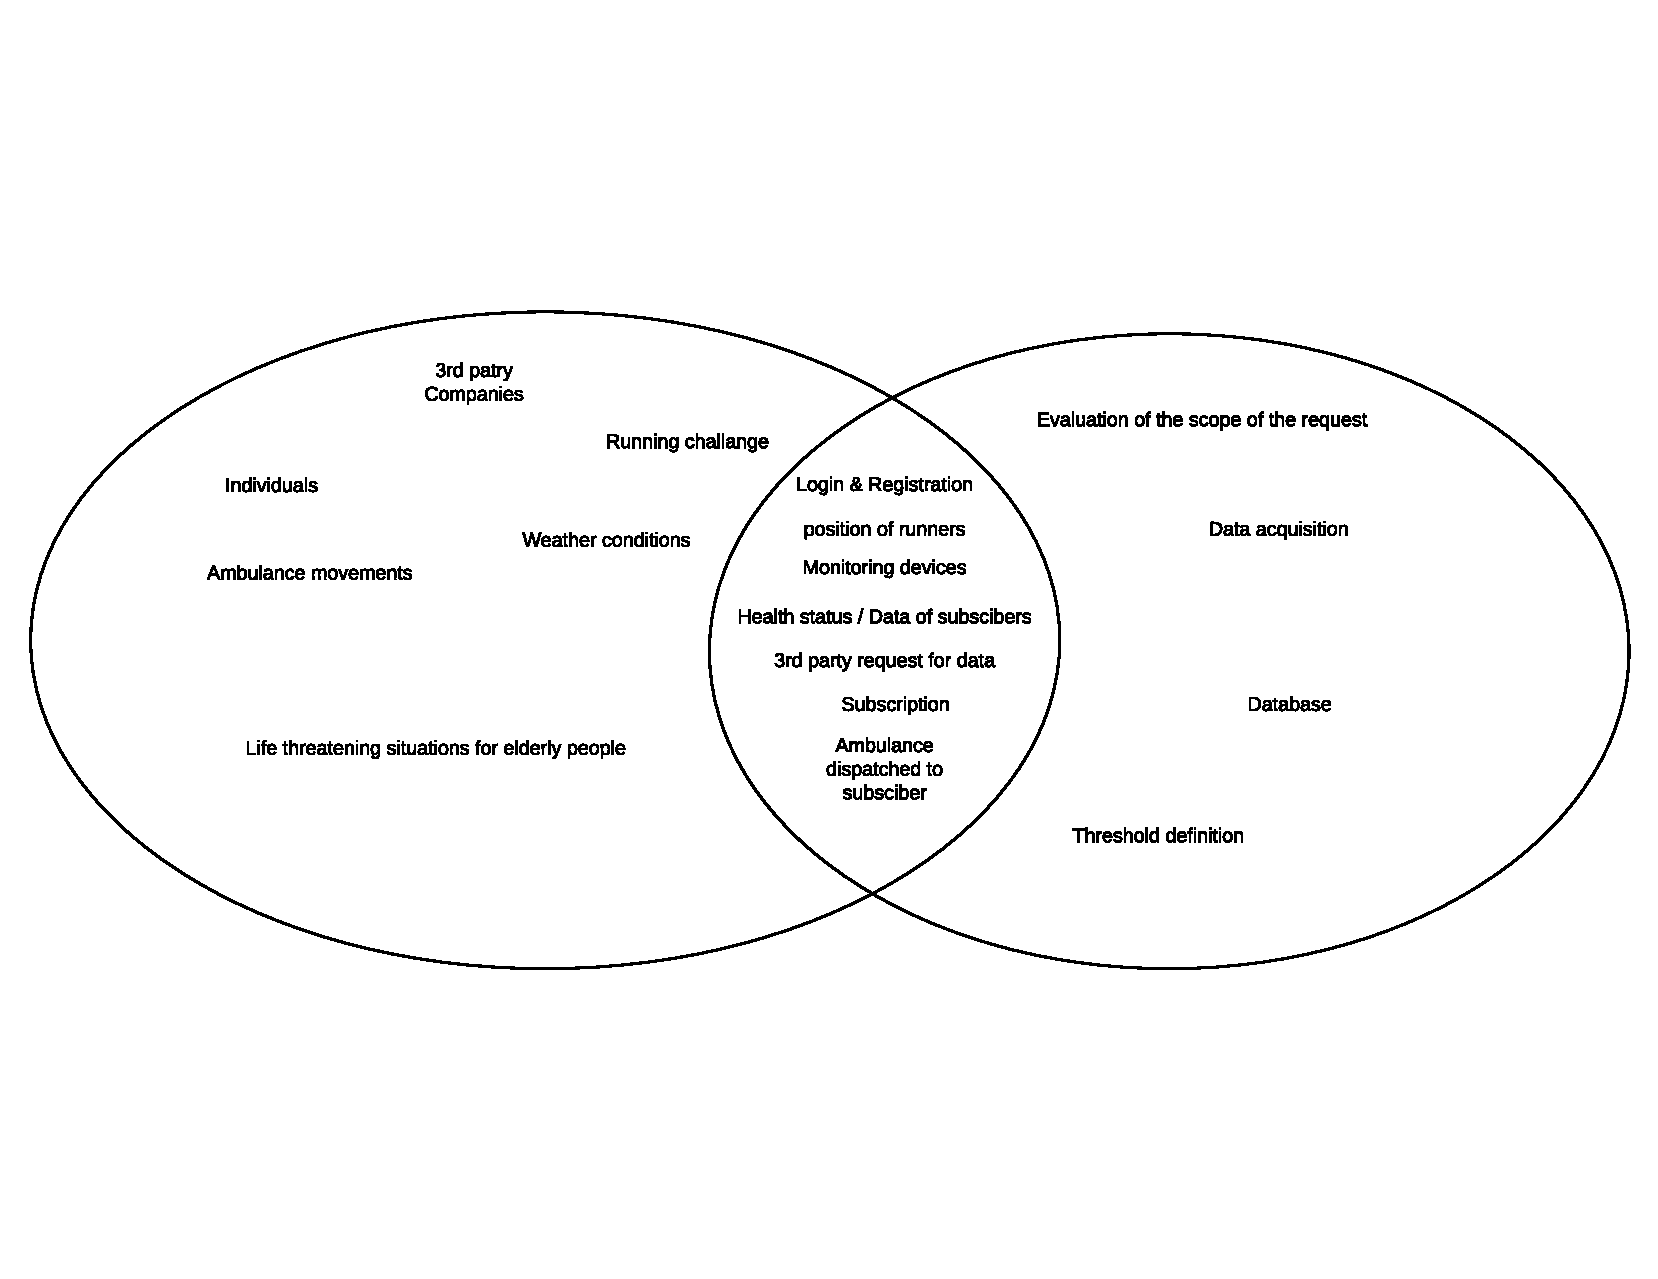
\includegraphics[height=8cm,keepaspectratio]{assets/twatm.pdf}
\end{center}

The system-to-be uses 3 components with different roles in order to work:
\begin{itemize}
    \item \textbf{Data4Help SmartWatch App}: Acquires the data from the smartwatch sensors (heart rate, sleep quality, position, phisical activities) and sends them via Bluetooth to the Data4Help Mobile App
    \item \textbf{Data4Help Mobile App}: Gathers data from the smartwatch, shows various statistics, and sends them to the Data4Help Core Database. Each user can choose which service subscribe to
    \item \textbf{Data4Help Website}: Gives third-party companies the ability to request data, either anonymized or user specific. Moreover, it allows run organizers to define the path of the run and the spectators to see the position of all runners on a map.
    \item \textbf{Data4Help Core}: is intended to connects all other components together providing the logic of the application. It is also responsible for the acceptance of all third-parties requests of data. It also evaluate health status of individuals deciding whether is at risk or not.
\end{itemize}

The list below shows the main goals the system should be able to accomplish:

\begin{itemize}
    \item \textbf{G1}: The system should be able to read sensor data from smart devices.
    \item \textbf{G2}: The system should be able to show acquired data via the Mobile App and the Website.
    \item \textbf{G3}: The system should allow users to register.
    \item \textbf{G4}: The system should allow companies to register.
    \item \textbf{G5}: The system should allow registered companies to request data either from specific individuals or from an anonymized group of individuals.
    \item \textbf{G6}: The system should allow users to accept or decline a company request for their specific data.
    \item \textbf{G7}: The system should provide a payment method to registered companies requesting user data. %eviterei di specificare payment system
    \item \textbf{G8}: The system should be able to communicate directly to ambulances.
    \item \textbf{G9}: The system should be able to react to the lowering of the health parameters below threshold in less than 5 seconds and send the position of the person to the ambulance system. 
    % \item \textbf{G10}: The system should should allow organizers to define the path for the run.
    \item \textbf{G10}: The system should be able to communicate interoperably with its services: \textit{AutomatedSOS} and \textit{Track4Run}
    \item \textbf{G11} The system should allow run organizers to register.
    \item \textbf{G12} If a run organizer is registered, it can define a run i.e. it can define the path that the participants should follow.
    \item \textbf{G13} A user should be able to enroll to a run.
    \item \textbf{G14} Spectators of a run should be able to see each participant's position on a map.
\end{itemize}

%A health data aggregator app that gives the user the ability to monitor all 

%is intended to offer all the functionalities of the service to the individuals, including heart rate monitoring, sleep monitoring




        \subsection{Definitions, Acronyms, Abbreviations}
            \renewcommand{\arraystretch}{1.5}
\begin{center}
    \begin{tabular}{|l|r|}
        \hline
        \textbf{i.e.} & \textit{Id est}, that is  \\
        \hline
        \textbf{w.r.t} & with respect to  \\
        \hline
        \textbf{w.l.o.g.} & without loss of generality \\
        \hline
        \textbf{The company} & TrackMe \\
        \hline
        \textbf{BLE} & Bluetooth Low Energy \\
        \hline
    \end{tabular}
\end{center}
        \subsection{Revision history}
        \subsection{Reference documents}
            \begin{itemize}
\item \textbf{|REFD1|} \href{https://en.wikipedia.org/wiki/Model–view–presenter}{\textbf{MVP}}

\item \textbf{|REFD2|} \href{https://standards.ieee.org/standard/1016-2009.html}{\textbf{IEEE Std 1016-2009 Standard for Information Technology, Systems Design, Software Design Descriptions}}

\item \textbf{|REFD3|} \href{https://it.wikipedia.org/wiki/Representational_State_Transfer}{\textbf{Representational State Transfers}}

\end{itemize}
        \subsection{Document structure}
        This document is divided in the following chapters:
\begin{description}
\item[Implemented requirements] Explains which functional requirements outlined in the RASD are accomplished, and how they are performed.
\item[Design choices] provides reasons about the implementation decisions taken in order to develop the application.
\item[Source code structure] explains and motivates how the source code is structured both in the front end and in the back end.
\item[Testing] provides the main testing cases applied to the the application
\item[REST API] describes the API implemented for the application.
\end{description}
    

\newpage
    \section{Implemented requirements}
    In this section there are described the functionalities implemented w.r.t the requirements listed in the RASD document.
Below there are listed all the functionality of the system, explained in terms of Database, Frontend, Backend handling.



\subsection{Actor Registration}
\begin{itemize}
\item \textbf{Implemented} requirements
        \begin{itemize}
   \item \textbf{[RM$_M$]}: Users can register, after providing a username, a password and a Fiscal Code/Social Security Number and have connected a compatible Smartwatch
    \item \textbf{[R2$_M$]}: Users can only have one account 
    
    %run organizer
  \item \textbf{[R11$_W$]}: Run organizers can register
    
    %company
    \item \textbf{[R1$_W$]}: Companies can register, after providing a username, a password, an email and a company name

%core
    \item \textbf{[R14$_C$]}: Can validates information provided by the user during registration

        \end{itemize}
    \item \textbf{Non-implemented} requirements
    \begin{itemize}
            \item 
        \end{itemize}
\end{itemize}

\paragraph{Database} \mbox{}\\ 
The database stores the actor data in the table "account".
Passwords are hashed and salted in order to avoid a security flaw.
The specific data for each type of actor is stored in specific tables, each for every actor type: individual\_account, company\_account, run\_organizer.
If the registering actor has, for instance, the same email of an actor already present on the database, the transaction is rolled back.
The same can be said for other \texttt{unique} parameters, such as the \texttt{SSN} for the \texttt{individual\_account}

\paragraph{Back-end} \mbox{}\\ 
The server first checks the required parameters for registration, depending on the actor, hashes the password and performs the first insertion into the table reserved for the actor (namely \texttt{individual\_account} \texttt{run\_organizer\_account} \texttt{company\_account}). Then generates a token which is stored and then sent to the actor mail in order to verify the account.
\paragraph{Front-end} \mbox{}\\

\begin{itemize}
    \item \textbf{Application}: 
    \item \textbf{Website}: Company can register through the homepage clicking on a button that opens a modal. After inserting the data, company clicks 'Send' and becomes automatically registered requiring an email verification.
\end{itemize}


\subsection{Actor Authentication}
\begin{itemize}
    \item \textbf{Implemented} requirements
        \begin{itemize}
    \item \textbf{[R1$_M$]}: Users can log-in
    
    %run organizer
    \item \textbf{[R12$_M$]}: Run organizers can login
    
    %company
    \item \textbf{[R2$_W$]}: Companies can log-in

%core

        \end{itemize}
    \item \textbf{Non-implemented} requirements
    \begin{itemize}
            \item 
        \end{itemize}
\end{itemize}

\paragraph{Database} \mbox{}\\ 
The given actor is requested from the database, if the comparison of the stored password and the given one is successful a token is inserted into the \texttt{user\_token} table.

\paragraph{Back-end} \mbox{}\\ 
The server checks the required parameters for the request, then proceedes to compare the hashed and non-hashed provided password. If the compare is successful it creates a token and stores it into the database, otherwise it negates the access to the actor.

\paragraph{Front-end} \mbox{}\\

\begin{itemize}
    \item \textbf{Application}: The application contains, under each subsection, a Login form. The application validates the information, performs the query to the server and show the result of the login. Both Users (individuals) and Run Organizers can log in using the application.
    \item \textbf{Website}: Company can login through the homepage clicking on a button "Sign in" that opens a modal. After inserting the data, company clicks 'Send' and access to the dashboard of his account.
\end{itemize}

\subsection{Individuals Management}

\begin{itemize}
    \item \textbf{Implemented} requirements
        \begin{itemize}
    %individuals
      
    \item \textbf{[R6$_M$]}: Logged-in users can accept/decline a company individual monitoring request
   
   %core
    \item \textbf{[R2$_C$]}: Can send online notifications via email to all users
    

        \end{itemize}
    \item \textbf{Non-implemented} requirements
    \begin{itemize}
    
    
    %core
    \item \textbf{[R1$_C$]}: Can send online notifications via SMS to all users 
    \item \textbf{[R3$_M$]}: Logged-in users can edit their account info
    \item \textbf{[R5$_W$]}: Logged-in companies can update their account information
    \item \textbf{[R3$_C$]}: Can send online notifications via the Mobile app to its users
        \end{itemize}
    %company
    \item \textbf{[R3$_W$]}: Logged-in companies can see their history and account information
        
\end{itemize}

\paragraph{Database} \mbox{}\\
The authorizations for each individual monitoring request is stored in the table individual\_query, in the column "auth", which is boolean (true if accepted, false if rejected, null if not already evaluated).
Back-end accesses column "email" in table account in order to send emails to the users.


\paragraph{Back-end} \mbox{}\\
The \texttt{/queries/query/individual/pending} endpoint allows the user to accept or decline the pending monitoring request.
The server sends online notification to every actor when he registers, in order to verify the email, and to the company that has performed a query when new data are available.

\paragraph{Front-end} \mbox{}\\
\textbf{Application:} Individual users can accept or decline a company monitoring request by the section reachable through the navigation drawer in the Dashboard.\\
\textbf{Website:} Company can see all account information in the panel 'Account' accessible via the navbar through all the pages, after having logged in.\\

\subsection{Company plan subscription }
\begin{itemize}
    \item \textbf{Implemented} requirements
        \begin{itemize}
            \item 
        \end{itemize}
    \item \textbf{Non-implemented} requirements
    \begin{itemize}
    \item \textbf{[R8$_C$]}: Can provide a payment method for data requested by companies.
    \item \textbf{[R15$_C$]}: Can charge companies on their payment method respecting Track4Me pricing policy
        \end{itemize}
\end{itemize}

\paragraph{Database} \mbox{}\\ 
The server answers with the mockup.
\paragraph{Back-end} \mbox{}\\  
\paragraph{Front-end} \mbox{}\\
\textbf{Web site}: The user can see all subscription plan available by clicking in the panel 'Account' accessible via the nav bar through all the pages, after having logged in.
Company can start the purchasing process after clicking "Purchase" under the respective subscription plan.



\subsection{Data management}
\begin{itemize}
    \item \textbf{Implemented} requirements
        \begin{itemize}
    %smartwatch
    
    %core
        \item \textbf{[R4$_C$]}: Can save and store permanently user data
    \item \textbf{[R5$_C$]}: Can receive and store health parameters and geographical position of registered users
     \item \textbf{[R2$_S$]}: App can send data registered locally to Data4Help Mobile App

        \end{itemize}
    \item \textbf{Non-implemented} requirements
    \begin{itemize}
    %smartwatch
    \item \textbf{[R1$_S$]}: App can read data from sensor and store it locally.
     
      \item \textbf{[R5$_M$]}: Logged-in can specify the nature of the daily activities (i.e. running, biking, swimming, hiking)

        \end{itemize}
\end{itemize}

\paragraph{Database} \mbox{}\\  
User data is stored in the tables "accelerometer", "gps\_coordinates", "hear\_rate", "user\_data".


\paragraph{Back-end} \mbox{}\\  
The individual user can send his data via the {indiv/data} endpoint.
The server inserts the user data into the respective table, if well formatted.
Then proceedes to notify the company for new data if the user is in one of the previously posted query.

\paragraph{Front-end} \mbox{}\\
\textbf{Application:} The data is not actually read from the sensors but the app can generate dummy test data and send it to the server, by the Test option in navigator drawer in he Dashboard.\\
\textbf{Web site: }Company can see data relative to their queries or to their monitored individuals right after having performed a query, clicking in the link provided by the server that redirects the user to a XML file containing the data requested.


\subsection{Query management}
\begin{itemize}
    \item \textbf{Implemented} requirements
        \begin{itemize}
    %company
    \item \textbf{[R6$_W$]}: Logged-in companies can query on some group of individuals data
    \item \textbf{[R7$_W$]}: Registered companies can request access to data of individuals
    \item \textbf{[R8$_W$]}: Logged-in companies can access to an individual data, if the user has given approval
    \item \textbf{[R9$_W$]}: Logged-in companies can export data previously queried using Data4Help

    %core
    \item \textbf{[R6$_C$]}: Can execute queries of companies on individuals if the user has accepted the monitoring request from the company
    \item \textbf{[R7$_C$]}: Can execute queries of companies checking if the searches involve more than 1000 anonimyzed users 

        \end{itemize}
    \item \textbf{Non-implemented} requirements
    \begin{itemize}
            \item 
        \end{itemize}
\end{itemize}

\paragraph{Database} \mbox{}\\ 
General information of queries are saved in table "query", while in tables "query\_user", "radius\_query" and "general\_query" are saved the specific information of queries.
The list of users subjected to the query is stored in the \texttt{query\_user} table.

\paragraph{Back-end} \mbox{}\\  
First, the given query is performed to assess feasibility (i.e on a high enough number of user) and then it is inserted in the database.
The list of users subjected to the query is inserted into the database as well.

\paragraph{Front-end} \mbox{}\\
\textbf{Web site}: Company can perform a query for group of individuals in the panel 'Query' accessible via the navbar through all the pages, after having logged in.\\
In the Query page it will appear a button to start a query. When clicked, it opens a modal with all fields to filter query parameters.
If left empty, the filter is just ignored.\\
The user can click "send" in order to perform the query.\\
Same works for single individuals: a company can perform a query clicking in the panel 'Monitoring' accessible via the navbar.

\subsection{Query subscription}
\begin{itemize}
    \item \textbf{Implemented} requirements
        \begin{itemize}
 \item \textbf{[R6bis$_W$]}: Logged-in companies can subscribe to a query data
        \end{itemize}
    \item \textbf{Non-implemented} requirements
    \begin{itemize}
            \item 
        \end{itemize}
\end{itemize}


\paragraph{Database} \mbox{}\\
\paragraph{Back-end} \mbox{}\\


\paragraph{Front-end} \mbox{}\\
\textbf{Web site:} In order to subscribe to a query, a company can simply select the tick-box in the subscription tick-box in the form of the 'Query' panel.
Company can subscribe to a query of group of individuals only, since there is no need to subscribe to single individuals query.

\subsection{Race Management}
\begin{itemize}
    \item \textbf{Implemented} requirements
        \begin{itemize}
        %individuals
    \item \textbf{[R8$_M$]}: Logged-in users can register to a run before the start time
    \item \textbf{[R9$_M$]}: Logged-in users can see a run information
    \item \textbf{[R13$_M$]}: Logged-in run organizers can organize a run
    \item \textbf{[R14$_M$]}: Organizers of a run can define the path and additional information for that run

        \end{itemize}
    \item \textbf{Non-implemented} requirements
    \begin{itemize}
            \item \textbf{[R15$_M$]}: Organizers of a run can start the run
        \end{itemize}
\end{itemize}

\paragraph{Database} \mbox{}\\
Information about a run are stored in the table "run". The checkpoints of the run are saved in the table "run\_check\_point". The subscriptions of each individual to runs are stored in the table "run\_subscription";
\paragraph{Back-end} \mbox{}\\
The \texttt{/runs} endpoint gives the client a way to exploit the requirements specified.
More specifically: 
\begin{itemize}
    \item \textbf{[R8$_W$]}: \texttt{/runs/join} allows the user to join a run, if exists
    \item \textbf{[R9$_W$]}: \texttt{/runs/positions} allows the user to gather informations on the position of the runners in a given run, if exists
    \item \textbf{[R13$_W$]}  \textbf{[R14$_W$]}: \texttt{/runs/} allows a run organizer to create a run, specifying its path, if it is well formed
\end{itemize}
\paragraph{Front-end} \mbox{}\\
\textbf{Application:} The user can register to a nearby run by using the Track4Run functionality reachable from the Dashboard. Here the user can also see the run information. Run Organizers can create a new run from their control panel, clicking the plus icon and defining checkpoints. The run start automatically at the defined time.

\subsection{Users Spectating Race}
\begin{itemize}
    \item \textbf{Implemented} requirements
        \begin{itemize}
        
        %individuals
        
        \item \textbf{[R10$_M$]}: Logged-in users can see participant position on a map, if the run has started


        %core

    \item \textbf{[R13$_C$]}: Can send the position and rank of athletes during a run to spectator's devices.


        \end{itemize}
    \item \textbf{Non-implemented} requirements
    \begin{itemize}
\item \textbf{[R12$_C$]}: Can compute each athlete's rank in a run and send it to each user device.
        \end{itemize}
\end{itemize}

\paragraph{Database} \mbox{}\\
The positions of the users are retrieved exploiting Data4Help functionality, so the data is in the "gps\_coordinates" table.

\paragraph{Back-end} \mbox{}\\
The server requests the runners position from the database for the given run, if exists.

\paragraph{Front-end} \mbox{}\\
\textbf{Application:} The users can see the position of participants on a map by clicking on View on the Track4Run section in the dashboard.

    
\newpage

    \section{Design Choices}
    \subsection{Data Layer}
    In order to manage data for our system, according to  DD document, we needed a relational database.
We could choose any SQL database. 
We opted for \texttt{PostgreSQL} because of its:
\begin{itemize}
    \item stability;
    \item high scalability;
    \item being opensource;
    \item easy to set up and use;
    \item availability of libraries for many programming languages;
    \item possibility to obtain free instance on Heroku;
\end{itemize}

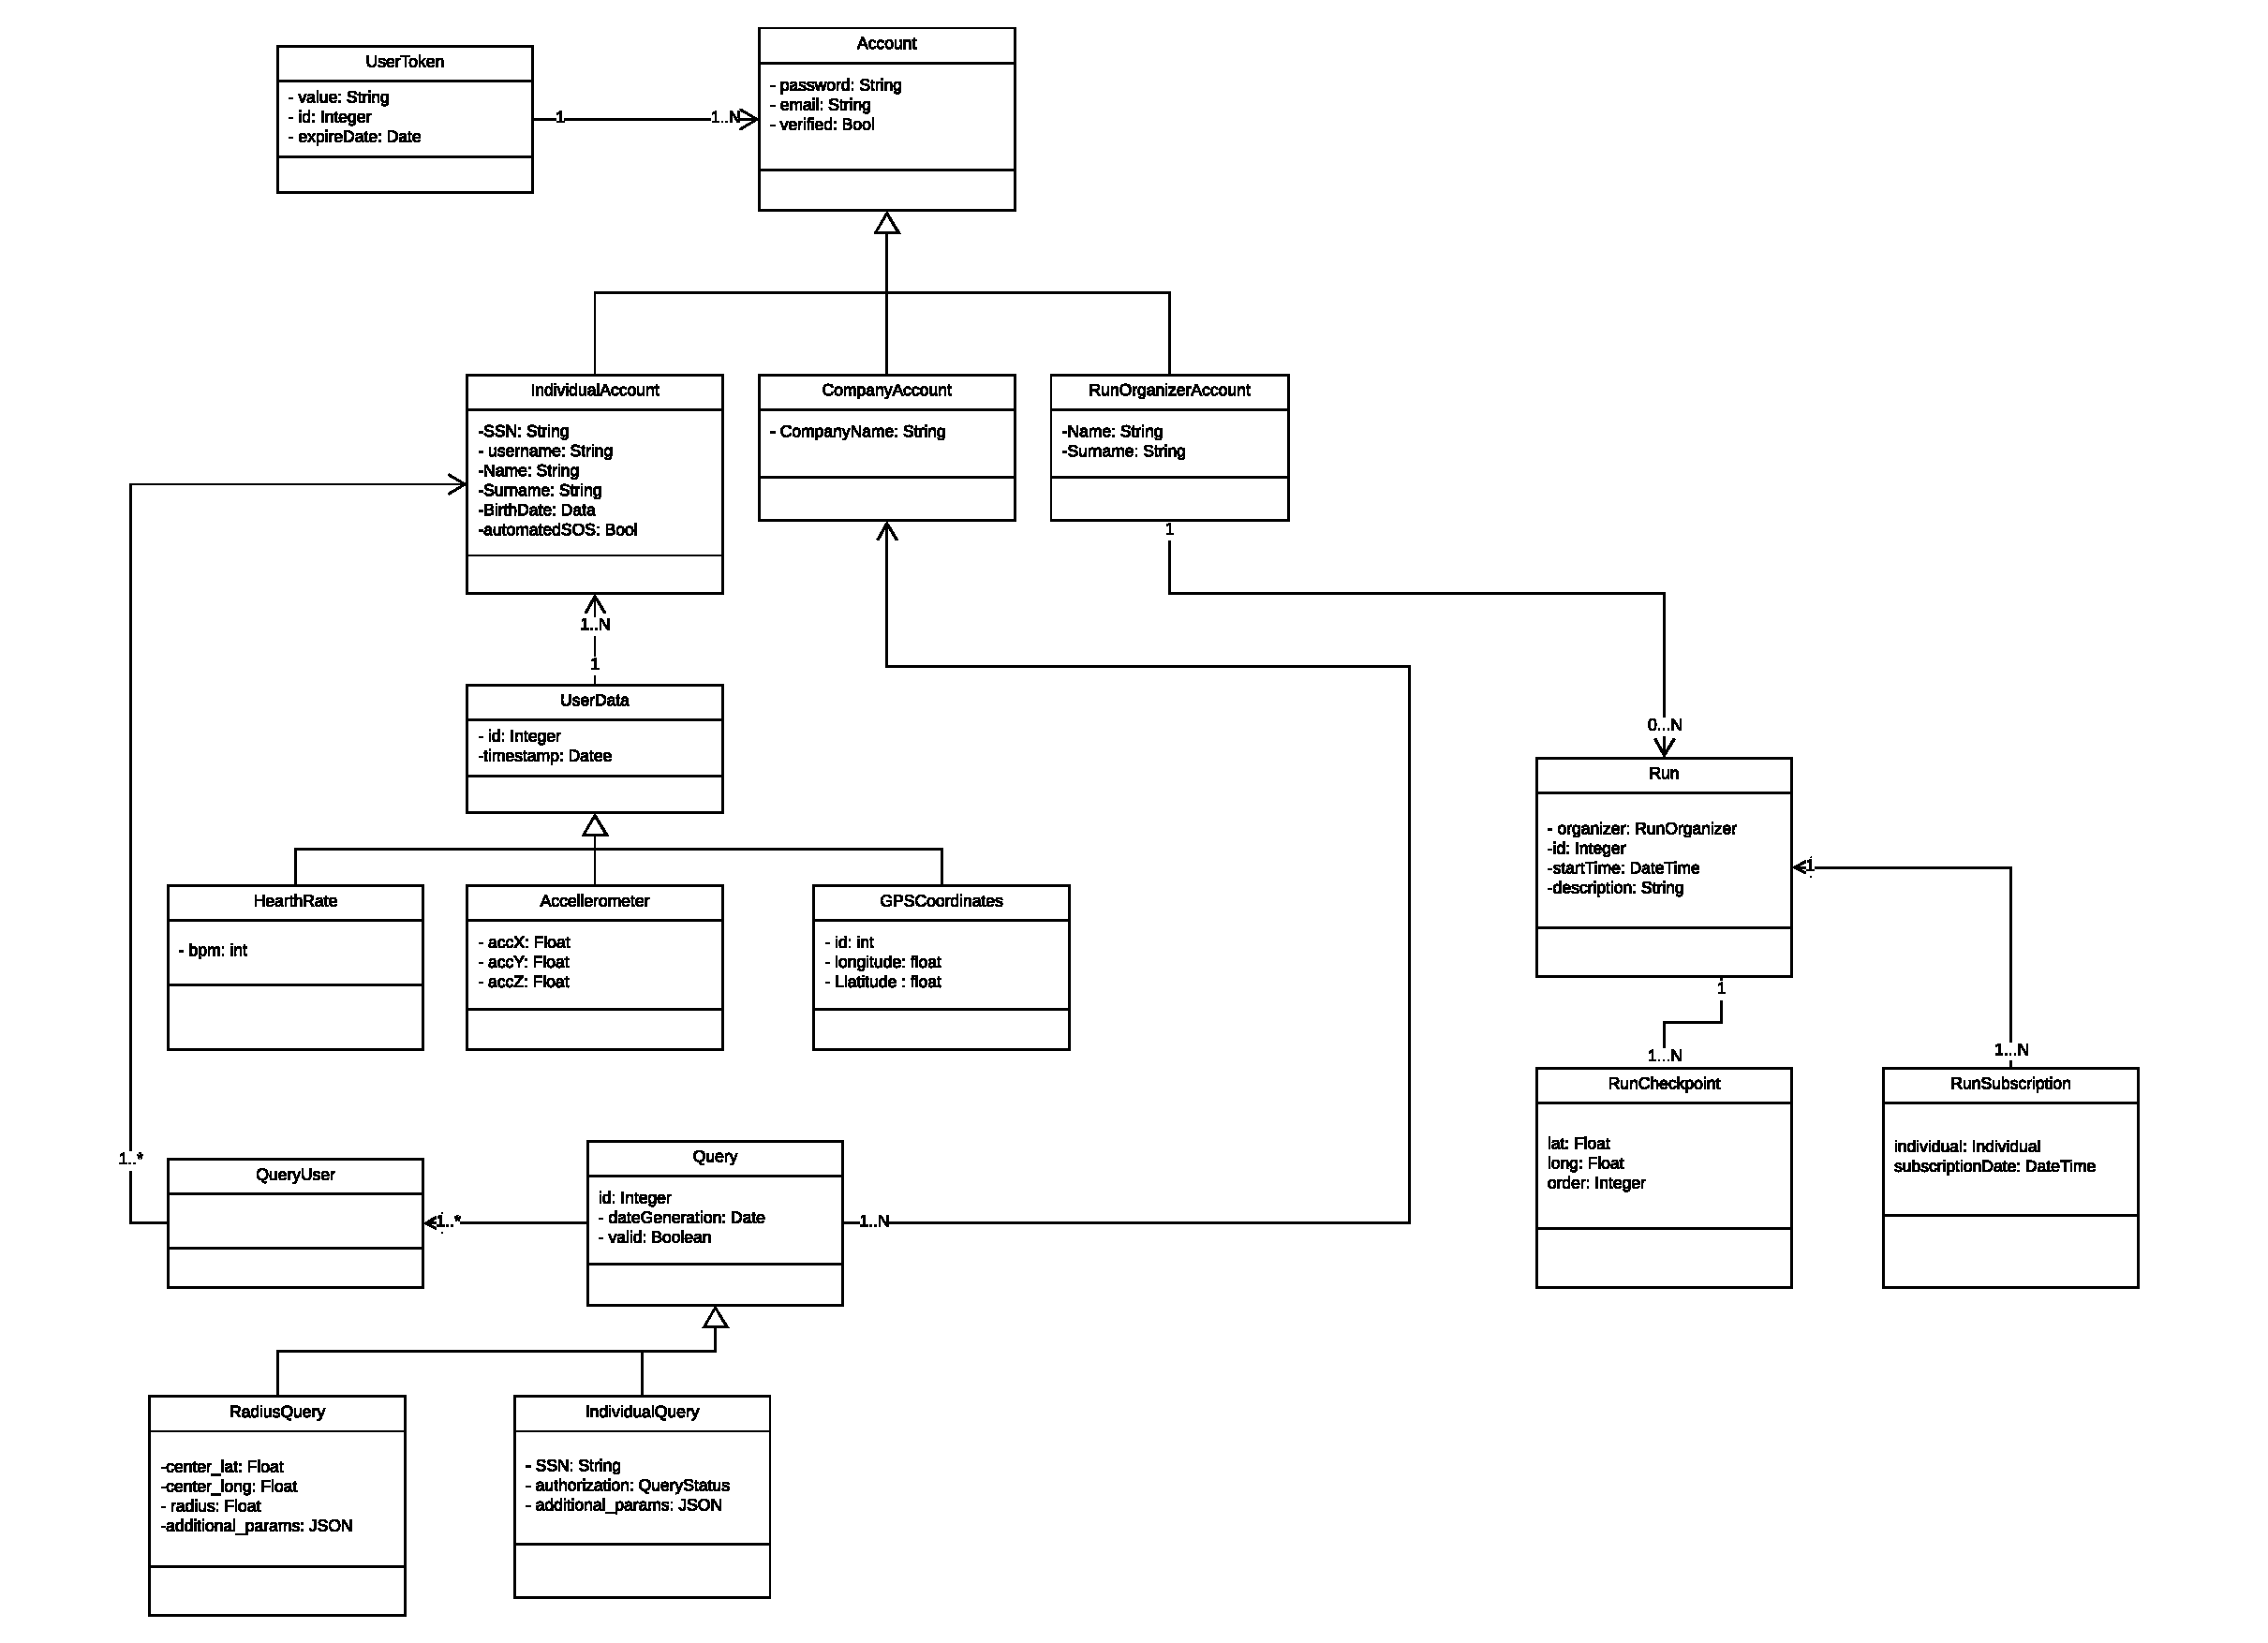
\includegraphics[width=\columnwidth]{assets/UML_Entities.pdf}
    \subsection{Business Logic Layer}
    \subsubsection{External services}
An external email service is used to send a verification email to each actor in order to verify the account.
Our system is email-provider independent, therefore it just needs the email, the password to be set via environmental variables.
See the insallation section for the details.

\subsubsection{Platform \& Used libraries}
\textbf{Nodejs}\\
\textbf{Nodejs} is a Javascript runtime.
This platform has been chosen because it is OS indipended, it offers many stable and well known libraries (ie \texttt{express} for the backend), it is well supported by the majority of the \textit{PAAS} and \textit{Heroku}, in our case. \\ Additionally its asynchronous handling of \textit{IO} has been proven to be fundamental for applications expecting high throughput. 
\vspace{1em} \\
\noindent \textbf{Libraries}\\
\textbf{Express} \\
Express is a \textit{Free and Open Source} web application framework that provides a robust set of features for building \textit{API}. Its functional approach in the use of middlewares and in routing (i.e. adding a new middleware to an \textit{endpoint} is done via adding one or multiple functions in the declaration of the endpoint) was proven to be critical to enhance the scalability of the code. Moreover the use of functions as middlewares provides great modularity to the application (i.e. adding and enpoint is done via adding a function in response to that route).
\vspace{0.5em}
\\
\textbf{Node Postgres} \\
Node Postgres is a collection of modules for interacting with the \texttt{PostgreSQL} database.
Due to the limitation imposed by \textit{Heroku PostgreSQL} (i.e. maximum of 20 active connections) it has been opted for this library as it provides an excellent pooling system, allowing the limiting of the maximum connection per pool. \\ Additionally it provides database \textit{Parametrized queries}, where the query string is passed directly to the database and parameters are substituted there instead of perform a string concatenation on the server, that could lead to an \textit{SQL Injection}.
\vspace{0.5em}
\\
\textbf{Security and Authentication}
\\
\textbf{BCrypt}\\
\textit{BCrypt} is the \textit{Javascript} implementation of the bcrypt hashing function based.
I provides a simple and criptographically secure way to hash password and compare them during authentication.\\
\vspace{0.5em}
\\
\textbf{JSONWebToken} \\
\textit{jsonwebtoken} is the \textit{javascript} implementation of the JSON Web Token Web standard. It provides a secure (\textit{URL Safe}) way to store user informations that need to be transferred between two parts. 
\vspace{0.5em}
\\
\textbf{Testing}\\
\textbf{Jest}\\
\textit{Jest} is an all in one 'zero configuration' testing platform. It provides simple methods to seamlessly test synchronous and asynchronous functions (which was mandatory for us) and either: 
\begin{itemize}
    \item Make an assertion on their output values
    \item Make an assertion on the resolving or rejection of an asynchronous function
    \item Make an assertion on the throwing of exception
\end{itemize}
Additionally, testing those three aspects is done similarly between synchronous and asynchronous functions, thus reducing the upfront setup code for the test.
    \subsection{Presentation Layer/Client}
    \subsubsection{Website}

\subsubsection{Mobile App}
\textbf{iOS / Android}
For the presentation layer, for what concerning the individual management and the run organizer part, we decided to build a native mobile app for the two main operating systems on the market, iOS and Android, using Flutter.
In this way we can cover about the 100\% of the market. [https://www.statista.com/statistics/266136/global-market-share-held-by-smartphone-operating-systems/]
Advantages of using Flutter are:
\begin{itemize}
    \item ability to share the same codebase between Android and iOS;
    \item ability to perform a fast development;
    \item the output is an app with native performance both on Android and iOS.
\end{itemize}

On the other hand, the Flutter project exited recently from the beta stage, and is in active development, but it's enough stable to be used in a production environment.

\textbf{Dart} Application built on Flutter needs to be written in Dart, which is a programming language designed by Google to let developers create high-quality, mission-critical apps for iOS, Android, and the web. It is an Object oriented programming language, which ereditates a lot from others programming language like Java, C\# and C++ in order to be very easy to learn.
It also support many new programming style, like the reactive programming, and support is strongly typed.

It compiles directly to native code (in case of Flutter) so that applications can run natively on devices, allowing a better management of resources and optimization of the subproducts of the compilation.
There are also a ton of different libraries that allow interoperability between Dart application and pre-existent software.

It is also free and open source.

\textbf{External libraries} The following external libraries have been used in order to add some functionality to the app. All the libraries are open source and publicly available from the Dart repository.
\begin{itemize}
    \item \textbf{google\_maps\_flutter}: allows to show a Google Map component in the app, which offers also the ability to place markers on it;
    \item \textbf{charts\_flutter}: allow to show chart of any type while being consistent with Material Design.
\end{itemize}


\textbf{External libraries} The following internal libraries have been used:
\begin{itemize}
    \item \textbf{http}: to make http/https queries to the backend,
    \item \textbf{material\_flutter}: offers the user interfaces main blocks, the widgets, in Material Design. It also manages all the life cycle of the app and the navigation in it.
\end{itemize}

\textbf{The MVP pattern} The Flutter application follows the MVP pattern that does not only define the actors of the app but also describe the way of how they communicate together. It consists of three components:
\begin{itemize}
    \item \textbf{Model}: it contains the logic that retrives the data that needs to be show to the user. It basically makes requests to the backend and decode the responses.
    \item \textbf{View}: it mains purpose is to show the data of the model to the user, formatted in an elegant way. It receives the user input and passes it to the Presenter.
    \item \textbf{Presenter}: it contains the business logic and manages the communications between the Model and the View, while keeping them completely separated.
\end{itemize}

Note that this is a \textit{thin client}, i.e. all the validation of the data inserted by the user is done mainly on the server. On the client side is done only the needed preprocessing for interoperability. 
    
\newpage
    \section{Source code structure}
    \subsection{Flutter project structure}
The following section's aim is to explain the structure of the Flutter project, that is the project for the Android/iOS frontend, managing the Individuals and Run Organizers operations.
This section only explains the content of every file but does not deep into details; for more information, please look at the source code.

This section will cover only the content \texttt{lib} folder, as the \texttt{android} and \texttt{ios} folder contain platform specific files, automatically generated by the Flutter project creator.

As stated before, the project is based on the MVP pattern and so the source code is organized in three folder, \texttt{model}, \texttt{view} and \texttt{presenter}. In this way it's more easy to maintain the code keeping the communication with the backend completely separated from the logic of the View.

\paragraph{Model}
The main aim of the model is to "hide" the retrieving of the new data from the server. It contains all the logic to interact with the server. In particular:
\begin{itemize}
    \item \texttt{UserModel.dart}: this is the actual model of the User. It contains all the necessary code to make HTTP request to the server to retrieve data and keeps track of the authentication code.
    \item \texttt{RunOrganizerModel.dart}: is the model of the Run Organizer. It contains the necessary code to retrieve the Run Organizer's details from the server and manage the auth code.
    \item \texttt{UserPersonalData.dart}: model for the user personal information. Contains the personal data of a user, like the name and the surname.
    \item \texttt{UserData.dart}: model for the user generated data. It contains the gps coordinates, the accelerometer information and data about heartRate. It also take care of decoding from and ancoding to the JSON format, in order to communicate with the server.
    \item \texttt{RunPoint.dart}: model for a single checkPoint in a Run.
    \item \texttt{Run.dart}: model for a Run. Contains information about the date and time of start and end, and the organizer.
    \item \texttt{PendingQueryRequest.dart}: model for individual requests of information. It contains the query id and the name of the Company.
\end{itemize}

\paragraph{Presenter}
The aim of the presenter is to take care of the interaction of the user with the View and react to them. It forwards all the request to the model, after doing some checks.
\begin{itemize}
    \item \texttt{UserPresenter.dart}: the presenter for the User model; it verifies the user input and if all is ok forwards the request to the model.
    \item \texttt{RunOrganizerPresenter.dart}: the presenter for the Run Organizer mdoel; it verifies the user input and if all is OK forwards the request to the model.
\end{itemize}

\paragraph{View} These are all the files under the View folder. Each files contains a specific screen of the application (or part of it). There are two main subfolder, one for each main part of te app.

For what concerning \textit{data4help}:
\begin{itemize}
    \item \texttt{CheckSmartwatchConnection.dart}: simulates the verification of the connection of a correct Smartwatch. If found sends the user to the login screen.
    \item \texttt{Data4HelpLogin.dart}: allows the user to insert its email and password and login, or to go to registration page if it does not have an account.
    \item \texttt{Data4HelpRegister.dart}: allows an unregistered user to register a new account.
    \item \texttt{Dashboard.dart}: multipage activity that allows the user to view and manage its infromation.
    \item \texttt{dashboard/DashboardMainPage.dart.dart}: shows to the user a recap on its daily activities.
    \item \texttt{dashboard/DashboardDetailPage.dart}: shows to the user a detailed page containing its daily activity. Allow the user to load a specific day.
    \item \texttt{dashboard/DashboardPendingQueriesRequests.dart}: shows to the user the pending requests for individual data by a Company. The user has the ability to accept or deny them.
    \item \texttt{dashboard/DashboardRunRegistrationPage.dart}: shows to the user the nearby runs and allow the Individual to subscribe to them if they are not started or to watch them of they are ongoing.
    \item \texttt{dashboard/DashboardTestPage.dart}: allows the user to send test data to the backend, simulating a connected smartwatch.
    \item \texttt{dashboard/WatchRun.dart}: shows the positions of the runners of a specific run on a map.
\end{itemize}

For what concerning \textit{track4run}:
\begin{itemize}
    \item \texttt{Track4RunLogin.dart}: allows the run organizer to insert its email and password and login, or to register if it does not have an account.
    \item \texttt{Track4RunRegister.dart}: allows an unregistered run organizer to register a new account.
    \item \texttt{DashboardRunOrganizer.dart}: shows to the run organizer all the run organized by him.
    \item \texttt{DashboardRunOrganizer.dart}: allows the run organizer tod efine a new run by specifying the details and the checkpoints.
    \item \texttt{DashboardRunOrganizer.dart}: allow he run organizer to add new checkpoint to the run.
\end{itemize}

\paragraph{Others files}
\begin{itemize}
    \item \texttt{Config.dart}: contains the global static configuration of the application, like the hostname of the backend.
    \item \texttt{Main.dart}: the main entry point of the app. It loads the first screen shown to the user.
\end{itemize}

\paragraph{App structure}
\begin{figure}[H]
	\includegraphics[width=\textwidth,height=\textheight,keepaspectratio]{assets/Android_App_Flow.pdf}
	\caption{Storyboard structure of the Mobile Application}
	\label{fig:StoryBoard}
\end{figure}
The figure above shows the UI flow of the app.
It is dived in four parts:
\begin{itemize}
    \item \textbf{Welcome page}: allows the user to access either the management part of the Individual or of the Runs;
    \item \textbf{Authentication and registration}: allows the user to login and register (the upper part to the individual part, the lower part to run organizer part);
    \item \textbf{Individual management}: allow the user to access its information, send and retrieve its data, join a run and view position of the runners in an ongoing run.
    \item \textbf{Run organizer management}: allows the run organizer to access information about its organized run and create new runs.
\end{itemize}




\subsection{Website structure}
This section aims explaining the structure of the web page into the website directory.
\vspace{4mm}
\\ The website  directory contains 3 sub-folders
\begin{itemize}
    \item CSS: contains the css configuration standardized by Materialized
    \item js: it contains only the initial file of the Materialized scripts. All other scripts are inside the html files.
    \item images: The images used for the graphic design. Contains the picture for parallax and the icons for data collection of queries performed.
\end{itemize}

Moreover, the website directory contains the html files describing the pages of the website.
The following lists only explain the content of the html files and what do they provide to the users. \\In order to see detailed information about the code, please look into the files themselves.

\subsubsection{Html files}
\begin{itemize}
    \item \textit{index.html} this is the Homepage of the website where user is re-directed if not logged-in.
    It contains a navbar where are shown the pages accessible for all not-logged users and a brief description of the data4Help services.
    Through the navbar are accessible the buttons for signin and signup. 
    \item \textit{services.html} this is the page that describes the services of Data4Help accessible through the website.
    It contains a navbar where are shown the pages accessible for all not-logged users and a brief description of the data4Help services.
    Through the navbar are accessible the buttons for signin and signup. 
    \item verify-email.html this is the page where a user is redirected after having successfully signed-up.
    It contains a navbar where are shown the pages accessible for all not-logged users and a brief description of the data4Help services.
    Through the navbar are accessible the buttons for signin and signup. 
    \item registration\_success.html this is the page where a user is re-directed after having verified his email.
    It contains a navbar where are shown the pages accessible for all not-logged users and a brief description of the data4Help services.
    Through the navbar are accessible the buttons for signin and signup. 
    \item \textit{dashboard.html} This is the dashboard of the website.
    A user who still has an session (i.e. having a valid auth\_token in the cookies) is re-directed in this page.
    The page shows the last 5 queries performed on a group of individuals by the company (if any).
    It contains a navbar where are shown the pages accessible for all logged users.
    Through the navbar are accessible a button for signout.
    \item \textit{monitoring.html} this is the core page of the individual queries.
    It lists all the queries of individuals performed by the company (if any) and let it download the content in any time by clicking to the button "Download query".
    It contains a navbar where are shown the pages accessible for all not-logged users and a brief description of the data4Help services.
    Through the navbar are accessible a button for signout.
    \item \textit{query.html} this is the core page of the queries for group of individuals.
    It lists all the queries for group of individuals performed by the company (if any) and let it download the content in any time by clicking to the button "Download query".
    It contains a navbar where are shown the pages accessible for all not-logged users and a brief description of the data4Help services.
    Through the navbar are accessible a button for signout.
    \item \textit{subscription.html} This is the page where a company can subscribe to a payment plan.
    However, this implementation it was not implemented and only displays the 3 possible subscription plan that respects the "Pricing Policies" described in the RASD document.
    It contains a navbar where are shown the pages accessible for all logged users.
    Through the navbar are accessible a button for signout.
\end{itemize}

\subsubsection{Javascript files}
\begin{itemize}
    \item \textit{materialize.js} contains default initialization provided by Materialize
    \item \textit{cookie-management.js} contains scripts that add/eliminate/update cookies of the user.
    \item \textit{query-list-retrieval.js} contains the scripts that retrieves the list of queries performed by the logged user.
    \item \textit{query-post.js} contains the scripts that permit users to perform a query for individuals and a query for radius search of group of individuals.
    \item \textit{signin-signout-modal.js} contains the scripts that manages the modals for signin and signup.
    \item \textit{signout-modal.js} contains the scripts that manages the modals for signout.
    \item \textit{switch-management.js}\textit{} contains the scripts managing the switch component for keeping company subscribed to a query (even if unsubscription was not implemented).
    \item \textit{xml-download-management.js} contains the scripts that manage the download of a query content returned by the server.
\end{itemize}

\paragraph{Website structure}
\begin{figure}[H]
	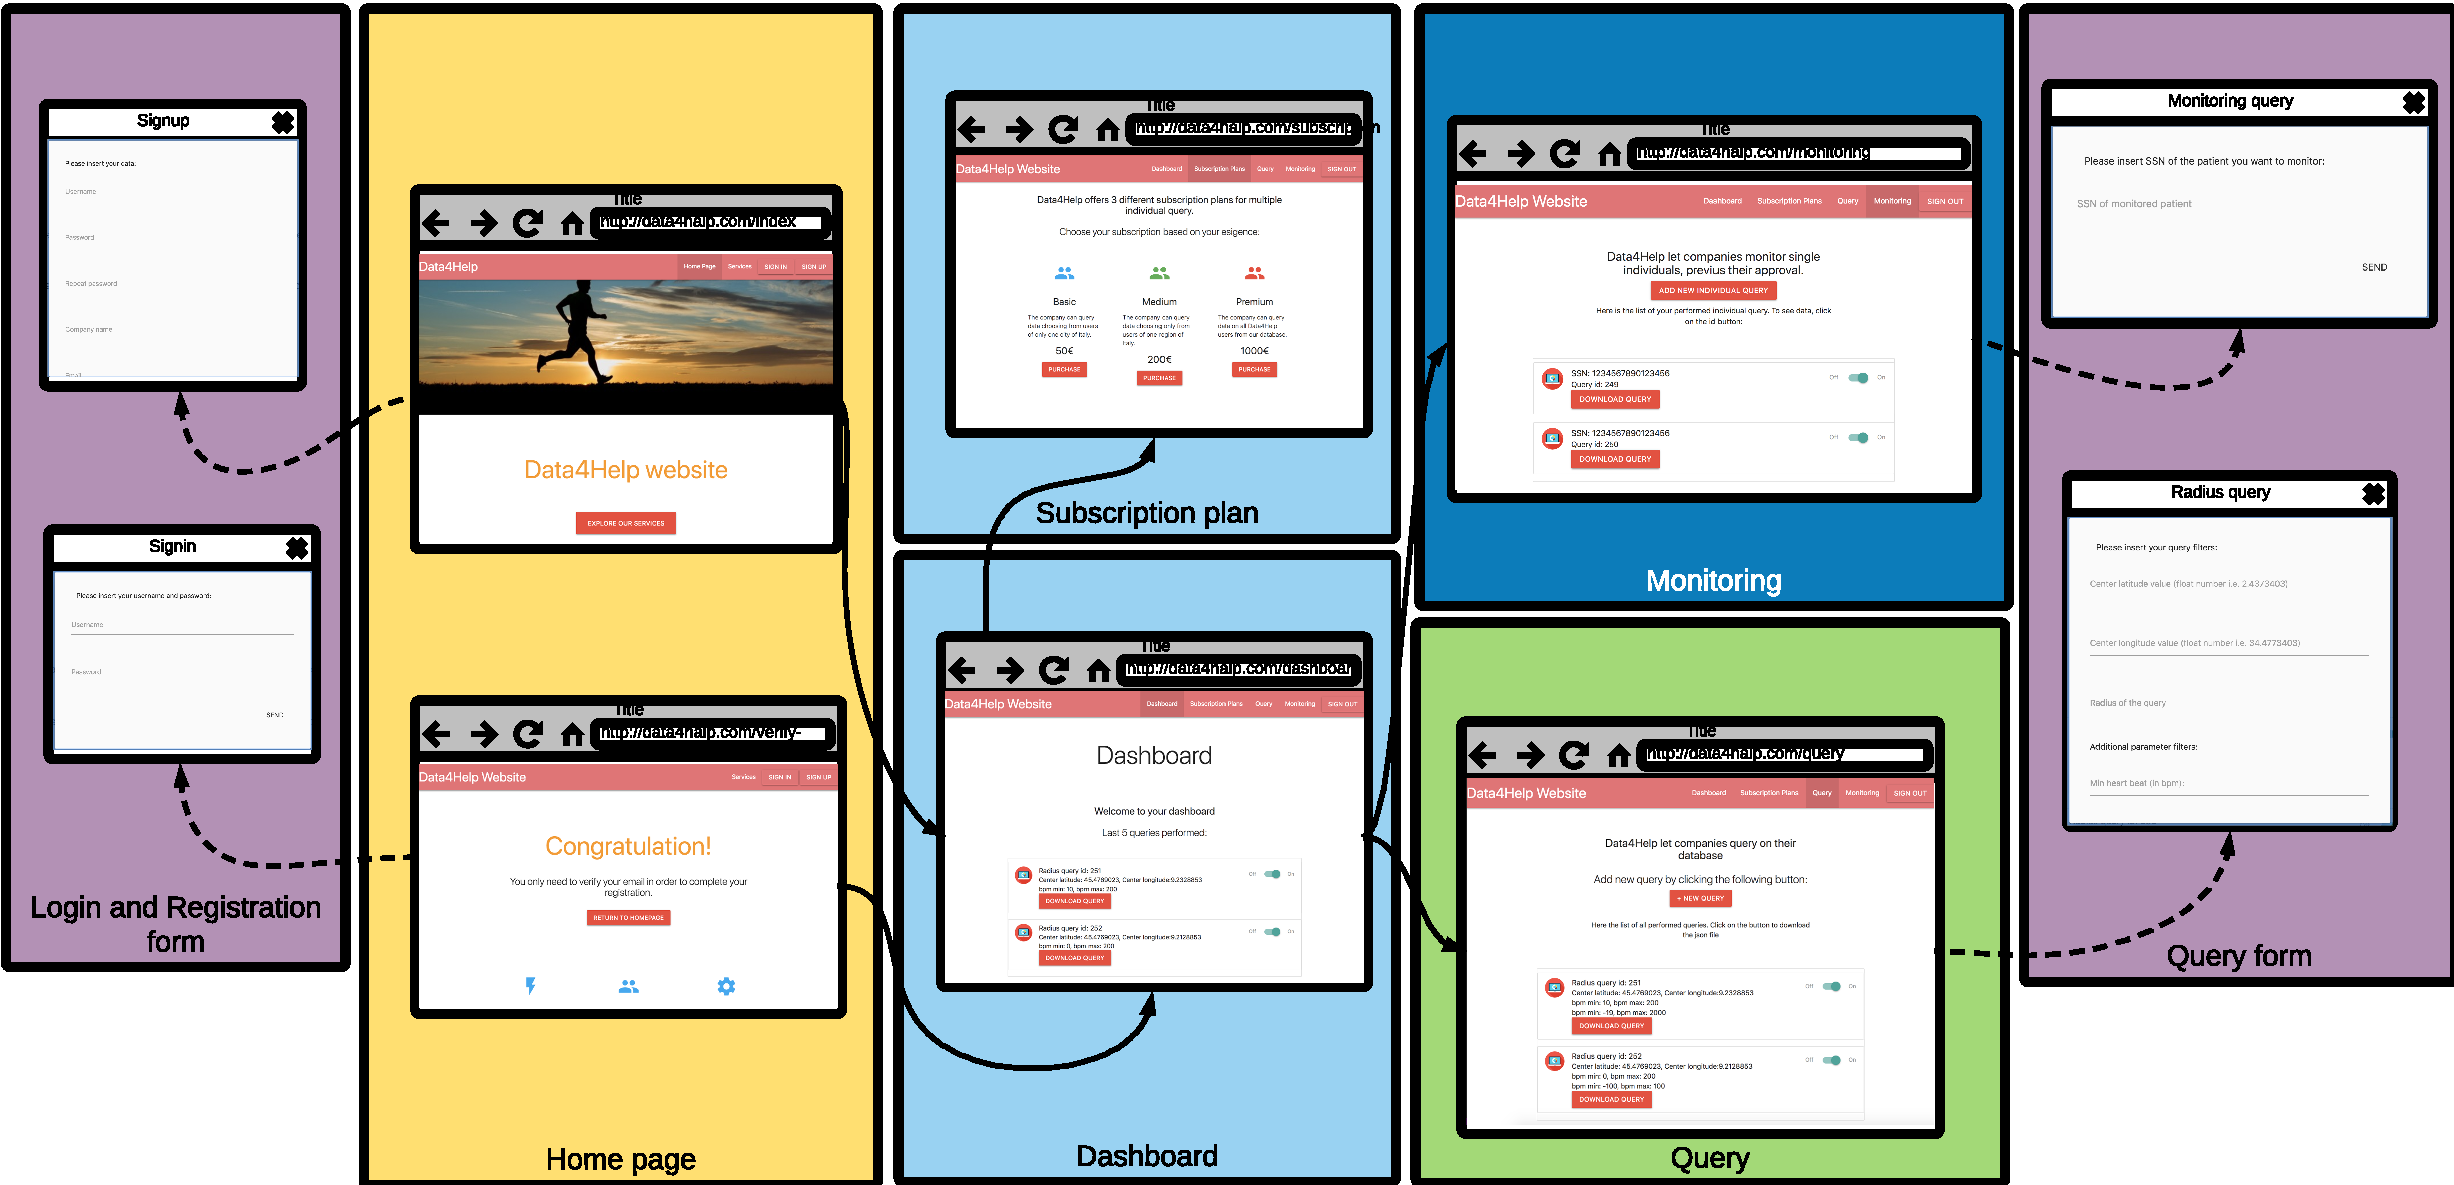
\includegraphics[width=\textwidth,height=\textheight,keepaspectratio]{assets/Website_Flow.pdf}
	\caption{Storyboard structure of the Website}
	\label{fig:StoryBoard}
\end{figure}
The figure above shows the UI flow of the website.
It is dived in four parts:
\begin{itemize}
    \item \textbf{Home page}: allows the user to either login or sign up. If correctly signed up, shows a successful registration page;
    \item \textbf{Login and Registration form}: the forms that user compiles in order to register.
    \item \textbf{Dashboard}: the page where the user is redirected after correct login;
    \item \textbf{Query}: allows the company to perform a new query on a group of individual and to download the xml of the already performed queries.
    \item \textbf{Monitoring}: allows the company to perform a new query on individuals and to download the XML content of the already performed queries.
    \item \textbf{Query form}: the forms that user compiles in order to perform queries.

\end{itemize}



\subsection{Backend project structure}
This section aims at explaining the structure of the backend inside the \texttt{backend} directory.
Note that this section only briefly describes the directories and the files in it, for more detailed explainations it is advisable to look at the comments in the source code.

The root directory contains the following files: 
\begin{itemize}
    \item \texttt{app.js} The entry point of the app. It defines how to handle different endpoints, how to catch errors and starts the server.
    \item \texttt{dbdump} Current dump of the database.
    \item \texttt{start.sh} Start script.
    \item \texttt{jest.config.js} The configuration file for \texttt{jest}, the testing framework.
    \item \texttt{package.json} Lists all the dependencies needed for the program to run and various other informations on the application.
    \item \texttt{package-lock.json} Contains the state of the dependency tree of the application.
    \item  \texttt{Procfile} Contains the command to be run by Heroku to start the application.
\end{itemize}
And the following directories: 
\begin{itemize}
    \item \texttt{managers}: Contains the managers of the application.
    \item \texttt{routes}: Contains the routes definition for the application.
    \item \texttt{\_\_tests\_\_}: Contains the tests for the application. 
    \item \texttt{utils}: Contains some utilites function used during testing and debugging
    \item \texttt{stub\_endpoint}: Contains the stub of endpoint responses used during the initial phase of building the application.
    All the responses contain a success response and various error responses.
\end{itemize}

\subsubsection{managers}
The managers folder contains a single file: 
\begin{itemize}
    \item \texttt{config.js}: Allows to configure some parameters of the app, such as the minimum number of users for which allow a radius query, the database to connect to and the maximum amount of client allowed.
\end{itemize}

And the following folders with their respective files \\
\noindent \textbf{authentication}
\begin{itemize}
    \item \texttt{AuthenticationManager.js}: Handles login and registration of actors.
    \item \texttt{requiredParams.json}: Required parameters for login and registration of each actor.
\end{itemize}

\noindent \textbf{individual}
\begin{itemize}
    \item \texttt{IndividualsManager.js}: Handles post and retreival of individuals' data.
    \item \texttt{requiredParams.json}: Required parameters for the data posted.
\end{itemize}

\noindent \textbf{query}
\begin{itemize}
    \item \texttt{QueriesManager.js}: Handles post, retreival and performing of the companies' queries.
    \item \texttt{requiredParams.json}: Required parameters for the queries.
    \item \texttt{templateQueries.json}: Template queries for insertion in the database 
\end{itemize}

\noindent \textbf{runs}
\begin{itemize}
    \item \texttt{RunManager.js}: Handles creation, retrieval of a run, joining a run and monitoring participants in a run.
    \item \texttt{runStatus}: Exports the constans for the status of a run.
\end{itemize}

\noindent \textbf{subs}
\begin{itemize}
    \item \texttt{SubscriptionManager.js}: Handles the subscription. Not implemented.
\end{itemize}

\noindent \textbf{token}
\begin{itemize}
    \item \texttt{TokenManager.js}: Handles operations concerning the token, such as the retreival of the actor or the check of the presence of the user in a database.
\end{itemize}

\subsubsection{routes}
The routes folder contains a single file: 
\begin{itemize}
    \item \texttt{router.js}: Joins all the defined endpoints end exports the as a single endpoint.
\end{itemize}

\noindent And the folder \texttt{endpoints}, which contains the following files: 
\begin{itemize}
    \item \texttt{auth.js}: Exports the endpoints for authentication. Handles login and registration of actors via the use of the functions declared in the \texttt{AuthenticationManager.js} file.
    \item \texttt{indiv.js}: Exports the endpoints for the individual. Handles post and retrival of individuals' data via the functions declared in the \texttt{IndividualsManagers.js} file.
    \item \texttt{queries.js}: Exports the endpoints for the queries. Handles post and retrival of company queries via the functions declared in the \texttt{QueriesManager.js} file.
    \item \texttt{runs.js}: Exports the endpoints for the runs management.  Handles post and retrival of run organizers run, subscription of individuals to a run, monitoring of runners in a run via the functions declared in the \texttt{RunsManager.js} file.
    \item \texttt{subs.js}: Exports the endpoints for subscription to query plans. Not implemented.

\end{itemize}

\subsubsection{\_\_tests\_\_}
The routes folder contains a single file: 
\begin{itemize}
    \item \texttt{config.js}: Internal configuration for the tests. Exports the token for company, run organizer, individual their mail and their password. Additionally it exports the URL on which perform the tests.
\end{itemize}

\noindent And the following directories with their respective files: \\
\noindent \textbf{auth}
\begin{itemize}
    \item \texttt{featureTest.jest.js}: Feature tests for the /auth endpoint
    \item \texttt{unitTest.jest.js}: Unit tests for the helper functions of \texttt{AuthenticationManager.js}
\end{itemize}
\noindent \textbf{indiv}
\begin{itemize}
    \item \texttt{featureTest.jest.js}: Feature tests for the /indiv endpoint
    \item \texttt{unitTest.jest.js}: Unit tests for the helper functions of \texttt{IndividualsManager.js}
\end{itemize}
\noindent \textbf{query}
\begin{itemize}
    \item \texttt{featureTest.jest.js}: Feature tests for the /queries endpoint
    \item \texttt{unitTest.jest.js}: Unit tests for the helper functions of \texttt{QueriesManager.js}
\end{itemize}
\noindent \textbf{runs}
\begin{itemize}
    \item \texttt{featureTest.jest.js}: Feature tests for the /runs endpoint
    \item \texttt{unitTest.jest.js}: Unit tests for the helper functions of \texttt{RunsManager.js}

\end{itemize}


\subsubsection{stub\_endpoint}
Contains the following folders: 

\noindent \textbf{auth}
\begin{itemize}
    \item \texttt{login.json}: Mock response on enpoint \texttt{/auth/login}.
    \item \texttt{register\_company.json}: Mock response on enpoint \texttt{/auth/register\_company}.
    \item \texttt{register\_run\_organizer.json}: Mock response on enpoint \texttt{/auth/register\_run\_organizer}.
    \item \texttt{register\_user.json}: Mock response on enpoint \texttt{/auth/register\_user}.
    \item \texttt{verify.json}: Mock response on enpoint \texttt{/auth/verify}.

\end{itemize}

\noindent \textbf{indiv}
\begin{itemize}
    \item \texttt{data\_POST.json}: Mock response for the POST request on endpoint \texttt{/indiv/data}.
    \item \texttt{data\_GET.json}: Mock response for the GET request on endpoint \texttt{/indiv/data}.
\end{itemize}

\noindent \textbf{query}
\begin{itemize}
    \item \texttt{query\_POST.json}: Mock response for the POST request on endpoint \texttt{/queries/query}.
    \item \texttt{query\_GET.json}: Mock response for the GET request on endpoint \texttt{/queries/query}.
\end{itemize}


\noindent \textbf{runs}
\begin{itemize}
    \item \texttt{join.json}: Mock response for the POST request on endpoint \texttt{/runs/join}.
    \item \texttt{positions.json}: Mock response for the GET request on endpoint \texttt{/runs/positions}.
     \item \texttt{root.json}: Mock response for the POST request on endpoint \texttt{/runs/}.
    \item \texttt{run.json}: Mock response for the GET request on endpoint \texttt{/runs/run}.
\end{itemize}

\noindent \textbf{subs}
\begin{itemize}
     \item \texttt{plan\_GET.json}: Mock response for the POST request on endpoint \texttt{/subs/plan}. Still active.
    \item \texttt{plan\_POST.json}: Mock response for the POST request on endpoint \texttt{/runs/positions}.
\end{itemize}

\subsubsection{utils}
Contains a single file: 
\begin{itemize}
    \item \texttt{testUtils.js} Utilities function used during testing.
\end{itemize}



    
\newpage
\subsection{Rest API}
In the following paragraph are represented the Rest API.
The API path has been modified putting as prefix \texttt{/v1}. In this way, we can provide a kind of versioning of the API interface so that future releases won't interfere with previous ones.

The following API are also present in the DD, this paragraph aims to describe in much details the request data and of the response.


    \textbf{Authentication Manager}
    \begin{itemize}
        \item User Registration
    \end{itemize}
    \begin{adjustwidth}{1cm}{}
        \begin{longtable}{|c|l|}
            \hline
            \textbf{Endpoint} & /v1/auth/register\_user \\
            \hline
            \textbf{URL Params} &  \\
            \hline
            \textbf{Method} & \textbf{POST} \\
            \hline
            \textbf{Request Data} & mail: String \\
            &                 password: String \\
            &                 SSN: String \\
            &                 name: String \\
            &                 surname: String \\
            &                 birthday: Date \\
            &                 smartwatch: String \\
            \hline
            \textbf{Success Response} & code: \texttt{200 OK} \\
            &                           content: \\
            & \begin{minipage}[t]{0.5\textwidth}
                \begin{adjustwidth}{1.5cm}{}
                \begin{verbatim}
{
    "success": true, 
    "auth_code": ...
}
                \end{verbatim}
                \end{adjustwidth}
              \end{minipage} \\
              \hline
            \textbf{Error Response} & code: \texttt{422 UNPROCESSABLE ENTITY} \\
            &                         content: \\
            & \begin{minipage}[t]{0.7\textwidth}
                \begin{adjustwidth}{1.5cm}{}
                \begin{verbatim}
{
    success: false, 
    error: 'InfoNotValid',
    message: ...
}
                \end{verbatim}
                \end{adjustwidth}
                \texttt{message} can be one of the following: 
                \begin{itemize}
                    \item \texttt{Unsupported smartwatch}
                    \item \texttt{Mail already used}
                    \item \texttt{SSN not valid} \\
                \end{itemize}
              \end{minipage} \\
              \hline
            \textbf{Uses} & Allows the client to register a new User \\
            \hline
             \textbf{Request example}
             & POST /v1/auth/register\_user \\
             & content: \\
            & \begin{minipage}[t]{0.5\textwidth}
                \begin{adjustwidth}{1.5cm}{}
                \begin{verbatim}
mail: example@gmail.com
password: password
SSN: 0123456789012345
name: Nico
surname: Fossa
birthday: 1996-01-01
smartwatch: SonySmartwatch3
                \end{verbatim}
                \end{adjustwidth}
              \end{minipage} \\
              \hline
             \textbf{Response example} & 
              \begin{minipage}[t]{0.5\textwidth}
                \begin{adjustwidth}{1.5cm}{}
                \begin{verbatim}
{
    "success":true,
    "auth_token":"eyJhbGciOiJIUz..."
}

                \end{verbatim}
                \end{adjustwidth}
              \end{minipage} \\
              \hline
        \end{longtable}
    \end{adjustwidth}

    \begin{itemize}
        \item Company Registration
    \end{itemize}
    \begin{adjustwidth}{1cm}{}
        \begin{longtable}{|c|l|}
            \hline
            \textbf{Endpoint} & /v1/auth/register\_company \\
            \hline
            \textbf{URL Params} &  \\
            \hline
            \textbf{Method} & \textbf{POST} \\
            \hline
            \textbf{Request Data} & email: String \\
            &                 password: String \\
            &                 company\_name: String \\

            \hline
            \textbf{Success Response} & code: \texttt{200 OK} \\
            &                           content: \\
            & \begin{minipage}[t]{0.5\textwidth}
                \begin{adjustwidth}{1.5cm}{}
                \begin{verbatim}
{
    success: true, 
    auth_code: ...
}
                \end{verbatim}
                \end{adjustwidth}
              \end{minipage} \\
              \hline
            \textbf{Error Response} & code: \texttt{422 UNPROCESSABLE ENTITY} \\
            &                         content: \\
            & \begin{minipage}[t]{0.7\textwidth}
                \begin{adjustwidth}{1.5cm}{}
                \begin{verbatim}
{
    success: false, 
    error: 'InfoNotValid',
    message: ...
}
                \end{verbatim}
                \end{adjustwidth}
                \texttt{message} can be one of the following: 
                \begin{itemize}
                    \item \texttt{Email already in use}\\
                \end{itemize}
              \end{minipage} \\
              \hline
            \textbf{Uses} & Allows the client to register a new Company \\
            \hline
             \textbf{Request example}
             & POST /v1/auth/register\_company \\
             & content: \\
            & \begin{minipage}[t]{0.5\textwidth}
                \begin{adjustwidth}{1.5cm}{}
                \begin{verbatim}
{
    email: "Htower@Htower.com",
    "password": "2Cid34242j",
    "company_name": "H-Tower",
    "type": 'company'
}
                \end{verbatim}
                \end{adjustwidth}
              \end{minipage} \\
              \hline
             \textbf{Response example} & 
              \begin{minipage}[t]{0.5\textwidth}
                \begin{adjustwidth}{1.5cm}{}
                \begin{verbatim}
{
    "success":true, 
    "auth_code":"eyJhbGciOiJIUz..."
}
                \end{verbatim}
                \end{adjustwidth}
              \end{minipage} \\
              \hline
        \end{longtable}
    \end{adjustwidth}

\begin{itemize}
        \item Run Organizer Registration
    \end{itemize}
    \begin{adjustwidth}{1cm}{}
        \begin{longtable}{|c|l|}
            \hline
            \textbf{Endpoint} & /v1/auth/register\_run\_organizer \\
            \hline
            \textbf{Method} & \textbf{POST} \\
            \hline
            \textbf{URL Params} &  \\
            \hline
            \textbf{Request Data} & email: String \\
            &                 password: String \\
            &                 name: String \\
            &                 surname: String \\
            \hline
            \textbf{Success Response} & code: \texttt{200 OK} \\
            &                           content: \\
            & \begin{minipage}[t]{0.5\textwidth}
                \begin{adjustwidth}{1.5cm}{}
                \begin{verbatim}
{
    success: true, 
    auth_code: ...
}
                \end{verbatim}
                \end{adjustwidth}
              \end{minipage} \\
              \hline
            \textbf{Error Response} & code: \texttt{422 UNPROCESSABLE ENTITY} \\
            &                         content: \\
            & \begin{minipage}[t]{0.7\textwidth}
                \begin{adjustwidth}{1.5cm}{}
                \begin{verbatim}
{
    success: false, 
    error: 'InfoNotValid',
    message: ...
}
                \end{verbatim}
                \end{adjustwidth}
                \texttt{message} can be one of the following: 
                \begin{itemize}
                    \item \texttt{SSN not valid}\\
                \end{itemize}
              \end{minipage} \\
              \hline
            \textbf{Uses} & Allows the client to register a new run organizer \\
            \hline
             \textbf{Request example}
             & POST /v1/auth/register\_run\_organizer \\
             & content: \\
            & \begin{minipage}[t]{0.5\textwidth}
                \begin{adjustwidth}{1.5cm}{}
                \begin{verbatim}
mail: example.runorganizer@gmail.com
password: password
name: Nico
surname: Fossa
birthday: 1996-01-01
                \end{verbatim}
                \end{adjustwidth}
              \end{minipage} \\
              \hline
             \textbf{Response example} & 
              \begin{minipage}[t]{0.5\textwidth}
                \begin{adjustwidth}{1.5cm}{}
                \begin{verbatim}
{
    "success":true,
    "auth_token":"eyJhbGciOiJIUz..."
}
                \end{verbatim}
                \end{adjustwidth}
              \end{minipage} \\
              \hline
        \end{longtable}
    \end{adjustwidth}

    \begin{itemize}
        \item User Login
    \end{itemize}
    \begin{adjustwidth}{1cm}{}
        \begin{longtable}{|c|l|}
            \hline
            \textbf{Endpoint} & /v1/auth/login \\
            \hline
            \textbf{Method} & \textbf{POST} \\
            \hline
            \textbf{URL Params} &  \\
            \hline
            \textbf{Request Data} & email: String \\
            &                 password: String \\
            &                 type: String \\
            \hline
            \textbf{Success Response} & code: \texttt{200 OK} \\
            &                           content: \\
            & \begin{minipage}[t]{0.5\textwidth}
                \begin{adjustwidth}{1.5cm}{}
                \begin{verbatim}
{
    success: true, 
    auth_token: ...
}
                \end{verbatim}
                \end{adjustwidth}
              \end{minipage} \\
              \hline
            \textbf{Error Response} & code: \texttt{404 NOT FOUND} \\
            &                         content: \\
            & \begin{minipage}[t]{0.7\textwidth}
                \begin{adjustwidth}{1.5cm}{}
                \begin{verbatim}
{
    success: false, 
    error: 'UserNotFound' ,
    message: 'User does not exists'
}
                \end{verbatim}
                \end{adjustwidth}
                \par\noindent\rule{\textwidth}{1pt}
                \vspace{4pt}
              \end{minipage} \\
              & code: \texttt{403 FORBIDDEN} \\
            &                         content: \\
            & \begin{minipage}[t]{0.7\textwidth}
                \begin{adjustwidth}{1.5cm}{}
                \begin{verbatim}
{
    success: false, 
    error: 'InvalidCredentials' ,
    message: 'Invalid Credentials'
}
                \end{verbatim}
                \end{adjustwidth}
              \end{minipage} \\
              \hline
            \textbf{Uses} & Allows the client to login \\
            \hline
             \textbf{Request example}
             & POST /v1/auth/login \\
             & content: \\
            & \begin{minipage}[t]{0.5\textwidth}
                \begin{adjustwidth}{1.5cm}{}
                \begin{verbatim}
email: example@gmail.com
password: password
type: individual
                \end{verbatim}
                \end{adjustwidth}
              \end{minipage} \\
              \hline
             \textbf{Response example} & 
              \begin{minipage}[t]{0.5\textwidth}
                \begin{adjustwidth}{1.5cm}{}
                \begin{verbatim}
{
    "success":true,
    "auth_token":"eyJhbGciOiJIUz..."
}
                \end{verbatim}
                \end{adjustwidth}
              \end{minipage} \\
              \hline
        \end{longtable}
    \end{adjustwidth}
    
    \begin{itemize}
        \item Verify mail
    \end{itemize}
    \begin{adjustwidth}{1cm}{}
        \begin{longtable}{|c|l|}
            \hline
            \textbf{Endpoint} & /v1/auth/verify \\
            \hline
            \textbf{Method} & \textbf{GET} \\
            \hline
            \textbf{URL Params} & mail: String \\
            &                     code: String \\
            &                     type: String \\
            \hline
            \textbf{Request Data} & \\
            \hline
            \textbf{Success Response} & code: \texttt{200 OK} \\
            &                           content: \\
            & \begin{minipage}[t]{0.5\textwidth}
                \begin{adjustwidth}{1.5cm}{}
                \begin{verbatim}
{
    success: true, 
    message: email verified
}
                \end{verbatim}
                \end{adjustwidth}
              \end{minipage} \\
              \hline
            \textbf{Error Response} & code: \texttt{401 UNAUTHORIZED} \\
            &                         content: \\
            & \begin{minipage}[t]{0.7\textwidth}
                \begin{adjustwidth}{1.5cm}{}
                \begin{verbatim}
{
    success: false, 
    error: 'InvalidCode',
    message: 'Code is invalid'
}
                \end{verbatim}
                \end{adjustwidth}
              \end{minipage} \\
              \hline
            \textbf{Uses} & Allows verification of the account \\
            \hline
             \textbf{Request example}
             & POST /v1/auth/verify \\
             & content: \\
            & \begin{minipage}[t]{0.5\textwidth}
                \begin{adjustwidth}{1.5cm}{}
                \begin{verbatim}
?mail=example@gmail.com&code=
eyJhbGciOiJ...&type=individual
                \end{verbatim}
                \end{adjustwidth}
              \end{minipage} \\
            \hline
             \textbf{Response example} & 
              \begin{minipage}[t]{0.5\textwidth}
                \begin{adjustwidth}{1.5cm}{}
                \begin{verbatim}
{
    success: true, 
    message: email verified
}
                \end{verbatim}
                \end{adjustwidth}
              \end{minipage} \\
              \hline
        \end{longtable}
    \end{adjustwidth}
    
    \textbf{Individuals Manager}
    \begin{itemize}
        \item Data store
    \end{itemize}
    \begin{adjustwidth}{1cm}{}
        \begin{longtable}{|c|l|}
            \hline
            \textbf{Endpoint} & /v1/indiv/data \\
            \hline
            \textbf{Method} & \textbf{POST} \\
            \hline
            \textbf{URL Params} &  \\
            \hline
            \textbf{Request Data} & auth\_token: String \\
            &                 data: JSON < Array < JSON > > \\
            
            \hline
            \textbf{Success Response} & code: \texttt{200 OK} \\
            &                           content: \\
            & \begin{minipage}[t]{0.5\textwidth}
                \begin{adjustwidth}{1.5cm}{}
                \begin{verbatim}
{
    success: true, 
    message: 'Sync successful'
}
                \end{verbatim}
                \end{adjustwidth}
              \end{minipage} \\
              \hline
            \textbf{Error Response} & code: \texttt{422 UNPROCESSABLE ENTITY} \\
            &                         content: \\
            & \begin{minipage}[t]{0.7\textwidth}
                \begin{adjustwidth}{1.5cm}{}
                \begin{verbatim}
{
    success: false, 
    error: 'InvalidData',
    message: 'Data are invalid'
}
                \end{verbatim}
                \end{adjustwidth}
                \par\noindent\rule{\textwidth}{1pt}
                 \vspace{4pt}
              \end{minipage} \\
          &                         code: \texttt{400 BAD REQUEST} \\
          &                         content: \\
          & \begin{minipage}[t]{0.7\textwidth}
            \begin{adjustwidth}{1.5cm}{}
                \begin{verbatim}
{
    success: false, 
    error: 'InvalidToken',
    message: 'Token is invalid'
}
                \end{verbatim}
                \end{adjustwidth}
          \end{minipage} \\
              \hline
            \textbf{Uses} & Allows the client to store sensor data in the database \\
            \hline
             \textbf{Request example}
             & POST /v1/indiv/data \\
             & content: \\
            & \begin{minipage}[t]{0.5\textwidth}
                \begin{adjustwidth}{1.5cm}{}
                \begin{verbatim}
{
   "gps_coordinates":[
      {
         "lat":45.473641,
         "long":9.228704,
         "timestamp":"2018-01-01
                      T00:00:00Z"
      }
   ],
   "accelerometer":[
      {
         "acc_x":0.147145,
         "acc_y":0.016155,
         "acc_z":0.917696,
         "timestamp":"2018-01-01
                      T00:00:00Z"
      }
   ],
   "heart_rate":[
      {
         "bpm":82,
         "timestamp":"2018-01-01
                      T00:00:00Z"
      }
   ]
}
                \end{verbatim}
                \end{adjustwidth}
              \end{minipage} \\
              \hline
             \textbf{Response example} & 
              \begin{minipage}[t]{0.5\textwidth}
                \begin{adjustwidth}{1.5cm}{}
                \begin{verbatim}
{
    success: true, 
    message: 'Sync successful'
}
                \end{verbatim}
                \end{adjustwidth}
              \end{minipage} \\
              \hline
        \end{longtable}
    \end{adjustwidth}
    
    \begin{itemize}
        \item Data retrival
    \end{itemize}
    \begin{adjustwidth}{1cm}{}
        \begin{longtable}{|c|l|}
            \hline
            \textbf{Endpoint} & /v1/indiv/data \\
            \hline
            \textbf{Method} & \textbf{GET} \\
            \hline
            \textbf{URL Params} &  auth\_token: String \\
            & begin\_date: Date \\
            & end\_date: Date \\
            \hline
            \textbf{Request Data} &  \\
            \hline
            \textbf{Success Response} & code: \texttt{200 OK} \\
            &                           content: \\
            & \begin{minipage}[t]{0.5\textwidth}
                \begin{adjustwidth}{1.5cm}{}
                \begin{verbatim}
{
    success: true, 
    data: SensorsData
}
                \end{verbatim}
                \end{adjustwidth}
              \end{minipage} \\
              \hline
            \textbf{Error Response} & code: \texttt{400 BAD REQUEST} \\
            &                         content: \\
            & \begin{minipage}[t]{0.7\textwidth}
                \begin{adjustwidth}{1.5cm}{}
                \begin{verbatim}
{
    success: false, 
    error: 'InvalidToken',
    message: 'Token is invalid'
}
                \end{verbatim}
                \end{adjustwidth}
              \end{minipage} \\
              \hline
            \textbf{Uses} & Allows the client to retrive sensor data from the database \\
            \hline
   \textbf{Request example}
             & GET /v1/indiv/data \\
             & content: \\
            & \begin{minipage}[t]{0.5\textwidth}
                \begin{adjustwidth}{1.5cm}{}
                \begin{verbatim}
?auth_token=eyJhbGciOiJ...&begin_date=
2018-01-01&end_date=2018-01-01
                \end{verbatim}
                \end{adjustwidth}
              \end{minipage} \\
              \hline
             \textbf{Response example} & 
              \begin{minipage}[t]{0.5\textwidth}
                \begin{adjustwidth}{1.5cm}{}
                \begin{verbatim}
{
   "success":true,
   "data":{
      "gps_coordinates":[
         {
            "lat":45.473641,
            "long":9.228704,
            "timestamp":"2018-01-01T00:00:00Z"
         }
      ],
      "accelerometer":[
         {
            "acc_x":0.147145,
            "acc_y":0.016155,
            "acc_z":0.917696,
            "timestamp":"2018-01-01T00:00:00Z"
         }
      ],
      "heart_rate":[
         {
            "bpm":82,
            "timestamp":"2018-01-01T00:00:00Z"
         }
      ]
   }
}
                \end{verbatim}
                \end{adjustwidth}
              \end{minipage} \\
              \hline
       
        \end{longtable}
    \end{adjustwidth}
    
    \begin{itemize}
        \item User information retrival
    \end{itemize}
    \begin{adjustwidth}{1cm}{}
        \begin{longtable}{|c|l|}
            \hline
            \textbf{Endpoint} & /v1/indiv/user \\
            \hline
            \textbf{Method} & \textbf{GET} \\
            \hline
            \textbf{URL Params} &  auth\_token: String \\
            \hline
            \textbf{Request Data} &  \\
            \hline
            \textbf{Success Response} & code: \texttt{200 OK} \\
            &                           content: \\
            & \begin{minipage}[t]{0.5\textwidth}
                \begin{adjustwidth}{1.5cm}{}
                \begin{verbatim}
{
    success: true, 
    user: ...userInfo
}
                \end{verbatim}
                \end{adjustwidth}
              \end{minipage} \\
              \hline
            \textbf{Error Response} & code: \texttt{400 BAD REQUEST} \\
            &                         content: \\
            & \begin{minipage}[t]{0.7\textwidth}
                \begin{adjustwidth}{1.5cm}{}
                \begin{verbatim}
{
    success: false, 
    error: 'InvalidToken',
    message: 'Token is invalid'
}
                \end{verbatim}
                \end{adjustwidth}
              \end{minipage} \\
              \hline
              & code: \texttt{404 Not Found} \\
            &                         content: \\
            & \begin{minipage}[t]{0.7\textwidth}
                \begin{adjustwidth}{1.5cm}{}
                \begin{verbatim}
{
    success: false, 
    error: 'Not found',
    message: 'The user wasn't found'
}
                \end{verbatim}
                \end{adjustwidth}
              \end{minipage} \\
              \hline
            \textbf{Uses} & Allows the client to retrive user informations \\
            \hline
               \textbf{Request example}
             & GET /v1/indiv/user \\
             & content: \\
            & \begin{minipage}[t]{0.5\textwidth}
                \begin{adjustwidth}{1.5cm}{}
                \begin{verbatim}
auth_token: eyJhbGciOiJ...
                \end{verbatim}
                \end{adjustwidth}
              \end{minipage} \\
            \hline
             \textbf{Response example} & 
              \begin{minipage}[t]{0.5\textwidth}
                \begin{adjustwidth}{1.5cm}{}
                \begin{verbatim}
{
   "success":true,
   "user":{
      "email":"example@gmail.com",
      "verified":true,
      "ssn":"1234567890123456",
      "birth_date":"2018-12-27
                    T00:00:00.000Z",
      "automated_sos":false,
      "smartwatch":"TestSmartwatch1",
      "name":"Nico",
      "surname":"Fossa"
   }
}
                \end{verbatim}
                \end{adjustwidth}
              \end{minipage} \\
              \hline
       
        \end{longtable}
    \end{adjustwidth}
   \textbf{Query Manager}
    
    \begin{itemize}
        \item Query creation
    \end{itemize}
    \begin{adjustwidth}{1cm}{}
        \begin{longtable}{|c|l|}
            \hline
            \textbf{Endpoint} & /v1/queries/query \\
            \hline
            \textbf{URL Params} &  \\
            \hline
            \textbf{Request Data} & auth\_token: String \\
            &                 query: json \\
            \hline
            \textbf{Success Response} & code: \texttt{200 OK} \\
            &                           content: \\
            & \begin{minipage}[t]{0.5\textwidth}
                \begin{adjustwidth}{1.5cm}{}
                \begin{verbatim}
{
    success: true, 
	message: 'Query successfully posted'
}
                \end{verbatim}
                \end{adjustwidth}
              \end{minipage} \\
              \hline
            \textbf{Error Response} & code: \texttt{422 UNPROCESSABLE ENTITY} \\
            &                         content: \\
            & \begin{minipage}[t]{0.7\textwidth}
                \begin{adjustwidth}{1.5cm}{}
                \begin{verbatim}
{
    success: false, 
    error: 'QueryTooRestrictive',
    message: 'Query on too few users'
}
                \end{verbatim}
                \end{adjustwidth}
                \par\noindent\rule{\textwidth}{1pt}
                 \vspace{4pt}
              \end{minipage} \\
              &                     code: \texttt{400 BAD REQUEST} \\
              &                     content: \\
              & \begin{minipage}[t]{0.7\textwidth}
                \begin{adjustwidth}{1.5cm}{}
                \begin{verbatim}
{
    success: false, 
    error: 'BadQuery',
    message: 'Query is invalid'
}
                \end{verbatim}
                \end{adjustwidth}
                 \par\noindent\rule{\textwidth}{1pt}
                 \vspace{4pt}
              \end{minipage} \\
              &                     code: \texttt{400 BAD REQUEST} \\
              &                     content: \\
              & \begin{minipage}[t]{0.7\textwidth}
                \begin{adjustwidth}{1.5cm}{}
                \begin{verbatim}
{
    success: false, 
    error: 'InvalidToken',
    message: 'Token is invalid'
}
                \end{verbatim}
                \end{adjustwidth}
                \par\noindent\rule{\textwidth}{1pt}
                 \vspace{4pt}
              \end{minipage} \\
              &                     code: \texttt{402 PAYMENT REQUIRED} \\
              &                     content: \\
              & \begin{minipage}[t]{0.7\textwidth}
                \begin{adjustwidth}{1.5cm}{}
                \begin{verbatim}
{
    success: false, 
    error: 'PaymentRequired',
    message: 'Payment required'
}
                \end{verbatim}
                \end{adjustwidth}
              \end{minipage} \\
              \hline
            \textbf{Uses} & Allows the client to create a query \\
            \hline
               \textbf{Request example}
             & POST /v1/queries/query \\
             & content: \\
            & \begin{minipage}[t]{0.5\textwidth}
                \begin{adjustwidth}{1.5cm}{}
                \begin{verbatim}
{
    "auth_token": "eyJhbGciOiJIUz...",
    "query": {
      "type": 'radius',
      "center_lat": 45.4398241,
      "center_long": 39.2489133,
      "radius": 10,
      "additional_params": {
        "acceleromete"r: {
          "acc_x": [-10, 15]
        },
        "heart_rate": {
          "bpm": [120, 160 ]
        }
      }
    }
}
                \end{verbatim}
                \end{adjustwidth}
              \end{minipage} \\
              \hline
             \textbf{Response example} & 
              \begin{minipage}[t]{0.5\textwidth}
                \begin{adjustwidth}{1.5cm}{}
                \begin{verbatim}
{
    "success": true,
    "message": "Query successfully posted"
}
                \end{verbatim}
                \end{adjustwidth}
              \end{minipage} \\
              \hline
        \end{longtable}
    \end{adjustwidth} 
    
    \begin{itemize}
        \item Query Retrival
    \end{itemize}
    \begin{adjustwidth}{1cm}{}
        \begin{longtable}{|c|l|}
            \hline
            \textbf{Endpoint} & /v1/queries/query \\
            \hline
            \textbf{Method} & \textbf{GET} \\
            \hline
            \textbf{URL Params} &  auth\_token: String \\
            \hline
            \textbf{Request Data} & \\
            \hline
            \textbf{Success Response} & code: \texttt{200 OK} \\
            &                           content: \\
            & \begin{minipage}[t]{0.5\textwidth}
                \begin{adjustwidth}{1.5cm}{}
                \begin{verbatim}
{
    success: true, 
    queries: ...totalQueries
}
                \end{verbatim}
                \end{adjustwidth}
              \end{minipage} \\
              \hline
            \textbf{Error Response} & code: \texttt{400 BAD REQUEST} \\
              &                     content: \\
              & \begin{minipage}[t]{0.7\textwidth}
                \begin{adjustwidth}{1.5cm}{}
                \begin{verbatim}
{
    success: false, 
    error: 'InvalidToken',
    message: 'Token is invalid'
}
                \end{verbatim}
                \end{adjustwidth}
                 \vspace{4pt}
              \end{minipage} \\
              \hline
            \textbf{Uses} & Allows the client to retrive the queries created by a company \\
            \hline
                           \textbf{Request example}
             & GET /v1/queries/query \\
             & content: \\
            & \begin{minipage}[t]{0.5\textwidth}
                \begin{adjustwidth}{1.5cm}{}
                \begin{verbatim}
?auth\_token=sjHeGbeuUwj...\&query\_id=13 
                \end{verbatim}
                \end{adjustwidth}
              \end{minipage} \\
            \hline
             \textbf{Response example} & 
              \begin{minipage}[t]{0.5\textwidth}
                \begin{adjustwidth}{1.5cm}{}
                \begin{verbatim}
{
    "success":true,
    "queries":   {
    "individual":[{
    "id":249,
    "ssn":
    "1234567890123456",
    "auth":true,
    "additional_params":{
        "accelerometer":{
            "acc_x":[-19,2000]
            },
        "heart_rate":{
            "bpm":[10,200]
            }
        }
    "subscribed":false
    }]
}
                \end{verbatim}
                \end{adjustwidth}
              \end{minipage} \\
              \hline
 
        \end{longtable}
    \end{adjustwidth} 
    
    \begin{itemize}
        \item Perform Query
    \end{itemize}
    \begin{adjustwidth}{1cm}{}
        \begin{longtable}{|c|l|}
            \hline
            \textbf{Endpoint} & /v1/queries/query/data \\
            \hline
            \textbf{method} & \textbf{GET} \\
            \hline
            \textbf{URL Params} &  auth\_token: String \\
            &  query\_id: Integer \\
            \hline
            \textbf{Request Data} & \\
            \hline
            \textbf{Success Response} & code: \texttt{200 OK} \\
            &                           content: \\
            & \begin{minipage}[t]{0.5\textwidth}
                \begin{adjustwidth}{1.5cm}{}
                \begin{verbatim}
{
    success: true,
    data: ...
}
                \end{verbatim}
                \end{adjustwidth}
              \end{minipage} \\
              \hline
            \textbf{Error Response} & code: \texttt{400 BAD REQUEST} \\
              &                     content: \\
              & \begin{minipage}[t]{0.7\textwidth}
                \begin{adjustwidth}{1.5cm}{}
                \begin{verbatim}
{
    success: false, 
    error: 'InvalidToken',
    message: 'Token is invalid'
}
                \end{verbatim}
                \end{adjustwidth}
                \par\noindent\rule{\textwidth}{1pt}
                 \vspace{4pt}
              \end{minipage} \\
              \hline
            \textbf{Uses} & Allows the client to perform a query \\
            \hline
                           \textbf{Request example}
             & GET /v1/queries/query/data \\
             & content: \\
            & \begin{minipage}[t]{0.5\textwidth}
                \begin{adjustwidth}{1.5cm}{}
                \begin{verbatim}
?auth_token=eKdgNeIegO...&query_id=23
                \end{verbatim}
                \end{adjustwidth}
              \end{minipage} \\
            \hline
             \textbf{Response example} & 
              \begin{minipage}[t]{0.5\textwidth}
                \begin{adjustwidth}{1.5cm}{}
                \begin{verbatim}
{
    success: true, 
    data: {
    success: true,
    data: "accelerometer":[{"timestamp":"2019-01-07T00:00:00.000Z","acc_x":0.993751,"acc_y":0.444582,"acc_z":0.464703}..."
}
}
                \end{verbatim}
                \end{adjustwidth}
              \end{minipage} \\
              \hline
 
        \end{longtable}
    \end{adjustwidth} 
    
    
        \begin{itemize}
        \item (still) Unauthorized queries retrieval
    \end{itemize}
    \begin{adjustwidth}{1cm}{}
        \begin{longtable}{|c|l|}
            \hline
            \textbf{Endpoint} & /v1/queries/query/individual/pending \\
            \hline
            \textbf{Method} & \textbf{GET} \\
            \hline
            \textbf{URL Params} &  auth\_token: String \\
            \hline
            \textbf{Request Data} & \\
            \hline
            \textbf{Success Response} & code: \texttt{200 OK} \\
            &                           content: \\
            & \begin{minipage}[t]{0.5\textwidth}
                \begin{adjustwidth}{1.5cm}{}
                \begin{verbatim}
{
    success: true, 
    queries: ...queries
}
                \end{verbatim}
                \end{adjustwidth}
              \end{minipage} \\
              \hline
            \textbf{Error Response} & code: \texttt{400 BAD REQUEST} \\
              &                     content: \\
              & \begin{minipage}[t]{0.7\textwidth}
                \begin{adjustwidth}{1.5cm}{}
                \begin{verbatim}
{
    success: false, 
    error: 'InvalidToken',
    message: 'Token is invalid'
}
                \end{verbatim}
                \end{adjustwidth}
                 \vspace{4pt}
              \end{minipage} \\
              \hline
            \textbf{Uses} & Get unapproved individual querie \\
            \hline
                           \textbf{Request example}
             & GET /v1/queries/individual/pending \\
             & content: \\
            & \begin{minipage}[t]{0.5\textwidth}
                \begin{adjustwidth}{1.5cm}{}
                \begin{verbatim}
auth_token: eyJhbGciOiJ...
                \end{verbatim}
                \end{adjustwidth}
              \end{minipage} \\
            \hline
             \textbf{Response example} & 
              \begin{minipage}[t]{0.5\textwidth}
                \begin{adjustwidth}{1.5cm}{}
                \begin{verbatim}
{
   "success":true,
   "queries":[
      {
         "id":248,
         "company_name":"Company1"
      },
      {
         "id":253,
         "company_name":"Company2"
      },
      {
         "id":250,
         "company_name":"Company3"
      }
   ]
}
                \end{verbatim}
                \end{adjustwidth}
              \end{minipage} \\
              \hline
 
        \end{longtable}
    \end{adjustwidth}
    
    \begin{itemize}
        \item Allow/Negate individual query
    \end{itemize}
    \begin{adjustwidth}{1cm}{}
        \begin{longtable}{|c|l|}
            \hline
            \textbf{Endpoint} & /v1/queries/query/individual/pending \\
            \hline
            \textbf{Method} & \textbf{POST} \\
            \hline
            \textbf{URL Params} &  \\
            \hline
            \textbf{Request Data} &  auth\_token: String \\
            & query\_id: Integer \\
            & decision: Boolean \\
            \hline
            \textbf{Success Response} & code: \texttt{200 OK} \\
            &                           content: \\
            & \begin{minipage}[t]{0.5\textwidth}
                \begin{adjustwidth}{1.5cm}{}
                \begin{verbatim}
{
    success: true, 
    message: 'Response Saved'
}
                \end{verbatim}
                \end{adjustwidth}
              \end{minipage} \\
              \hline
            \textbf{Error Response} & code: \texttt{400 BAD REQUEST} \\
              &                     content: \\
              & \begin{minipage}[t]{0.7\textwidth}
                \begin{adjustwidth}{1.5cm}{}
                \begin{verbatim}
{
    success: false, 
    error: 'InvalidToken',
    message: 'Token is invalid'
}
                \end{verbatim}
                \end{adjustwidth}
                 \vspace{4pt}
              \end{minipage} \\
              \hline
            \textbf{Uses} & Specify decision for individual query \\
            \hline
            
            
                           \textbf{Request example}
             & POST /v1/queries/individual/pending \\
             & content: \\
            & \begin{minipage}[t]{0.5\textwidth}
                \begin{adjustwidth}{1.5cm}{}
                \begin{verbatim}
auth_token: eyJhbGciOiJ...
query_id: 21
decision: true
                \end{verbatim}
                \end{adjustwidth}
              \end{minipage} \\
            \hline
             \textbf{Response example} & 
              \begin{minipage}[t]{0.5\textwidth}
                \begin{adjustwidth}{1.5cm}{}
                \begin{verbatim}
{
   "success":true,
   "message":"Response saved"
}
                \end{verbatim}
                \end{adjustwidth}
              \end{minipage} \\
              \hline
 
 
        \end{longtable}
    \end{adjustwidth}
    
    
    \textbf{Subscription Manager}
    \begin{itemize}
        \item Buy subscription plan
    \end{itemize}
    \begin{adjustwidth}{1cm}{}
        \begin{longtable}{|c|l|}
            \hline
            \textbf{Endpoint} & /v1/subs/plan \\
            \hline
            \textbf{Method} & \textbf{POST} \\
            \hline
            \textbf{URL Params} &  \\
            \hline
            \textbf{Request Data} & auth\_token: String \\
            &                 mail: String \\
            &                 plan: String \\
            \hline
            \textbf{Success Response} & code: \texttt{200 OK} \\
            &                           content: \\
            & \begin{minipage}[t]{0.5\textwidth}
                \begin{adjustwidth}{1.5cm}{}
                \begin{verbatim}
{
    success: true, 
    message: {$PLAN} bought
}
                \end{verbatim}
                \end{adjustwidth}
                \par\noindent\rule{1.39\textwidth}{1pt}
                 \vspace{4pt}
              \end{minipage} \\
              &                     code: \texttt{400 BAD REQUEST} \\
              &                     content: \\
              & \begin{minipage}[t]{0.7\textwidth}
                \begin{adjustwidth}{1.5cm}{}
                \begin{verbatim}
{
    success: false, 
    error: 'InvalidToken',
    message: 'Token is invalid'
}
                \end{verbatim}
                \end{adjustwidth}
                \par\noindent\rule{\textwidth}{1pt}
                 \vspace{4pt}
              \end{minipage} \\
              &                     code: \texttt{402 PAYMENT REQUIRED} \\
              &                     content: \\
              & \begin{minipage}[t]{0.7\textwidth}
                \begin{adjustwidth}{1.5cm}{}
                \begin{verbatim}
{
    success: false, 
    error: 'PaymentRequired',
    message: 'Payment required'
}
                \end{verbatim}
                \end{adjustwidth}
                \par\noindent\rule{\textwidth}{1pt}
                 \vspace{4pt}
              \end{minipage} \\
              &                     code: \texttt{404 NOT FOUND} \\
              &                     content: \\
              & \begin{minipage}[t]{0.7\textwidth}
                \begin{adjustwidth}{1.5cm}{}
                \begin{verbatim}
{
    success: false, 
    error: 'PlanNotFound',
    message: 'Plan not found'
}
                \end{verbatim}
                \end{adjustwidth}
              \end{minipage} \\
              \hline
            \textbf{Uses} & Allows the client buy a subscription to a new plan \\
            \hline
          
        \end{longtable}
    \end{adjustwidth} 
    
    \begin{itemize}
        \item Get plan informations
    \end{itemize}
    \begin{adjustwidth}{1cm}{}
        \begin{longtable}{|c|l|}
            \hline
            \textbf{Endpoint} & /v1/subs/plan \\
            \hline
            \textbf{Method} & \textbf{GET} \\
            \hline
            \textbf{URL Params} &  plan: String \\
            \hline
            \textbf{Request Data} & \\
            \hline
            \textbf{Success Response} & code: \texttt{200 OK} \\
            &                           content: \\
            & \begin{minipage}[t]{0.5\textwidth}
                \begin{adjustwidth}{1.5cm}{}
                \begin{verbatim}
{
    success: true, 
    plan: ...planDetails
}
                \end{verbatim}
                \end{adjustwidth}
              \end{minipage} \\
              \hline
            \textbf{Error Response} & code: \texttt{400 BAD REQUEST} \\
            &                         content: \\
            & \begin{minipage}[t]{0.7\textwidth}
                \begin{adjustwidth}{1.5cm}{}
                \begin{verbatim}
{
    success: false, 
    error: 'PlanUnavailable',
    message: 'Plan is not available'
}
                \end{verbatim}
                \end{adjustwidth}
                \par\noindent\rule{1.2\textwidth}{1pt}
                 \vspace{4pt}
              \end{minipage} \\
              
              &                     code: \texttt{404 NOT FOUND} \\
              &                     content: \\
              & \begin{minipage}[t]{0.7\textwidth}
                \begin{adjustwidth}{1.5cm}{}
                \begin{verbatim}
{
    success: false, 
    error: 'PlanNotFound',
    message: 'Plan not found'
}
                \end{verbatim}
                \end{adjustwidth}
                
              \end{minipage} \\
              \hline
            \textbf{Uses} & Allows the client retrive informations about a subscription plan \\
            \hline
            

        \end{longtable}
    \end{adjustwidth}
    
    \textbf{Run Manager}
        \begin{itemize}
            \item Create a Run
        \end{itemize}
        \begin{adjustwidth}{1cm}{}
            \begin{longtable}{|c|l|}
                \hline
                \textbf{Endpoint} & /v1/runs/run \\
                \hline
                \textbf{Method} & \textbf{POST} \\
                \hline
                \textbf{URL Params} &  \\
                \hline
                \textbf{Request Data} & auth\_token: String \\
                &                 time\_begin: Date \\
                &                 time\_end: Date \\
                &                 description: String \\
                &                 coordinates: Array < JSON > \\
                \hline
                \textbf{Success Response} & code: \texttt{200 OK} \\
                &                           content: \\
                & \begin{minipage}[t]{0.5\textwidth}
                    \begin{adjustwidth}{1.5cm}{}
                    \begin{verbatim}
    {
        success: true, 
        run_id: $ID
    }
                    \end{verbatim}
                    \end{adjustwidth}
                  \end{minipage} \\
                  \hline
                \textbf{Error Response} & code: \texttt{422 UNPROCESSABLE ENTITY} \\
                &                         content: \\
                & \begin{minipage}[t]{0.7\textwidth}
                    \begin{adjustwidth}{1.5cm}{}
                    \begin{verbatim}
    {
        success: false, 
        error: 'InfoNotValid',
        message: ...
    }
                    \end{verbatim}
                    \end{adjustwidth}
                    \texttt{message} can be one of the following: 
                    \begin{itemize}
                        \item \texttt{Time not valid}
                        \item \texttt{Coordinates not valid}
                    \end{itemize}
                     \par\noindent\rule{\textwidth}{1pt}
                 \vspace{4pt}
                  \end{minipage} \\
                & code: \texttt{403 FORBIDDEN} \\
                &                         content: \\
                & \begin{minipage}[t]{0.7\textwidth}
                    \begin{adjustwidth}{1.5cm}{}
                    \begin{verbatim}
    {
        success: false, 
        error: 'InvalidCredentials',
        message: 'Invalid Credentials'
    }
                    \end{verbatim}
                    \end{adjustwidth}
                  \end{minipage} \\
                  \hline
                \textbf{Uses} & Allows the client to create a new run \\
                \hline
                
                               \textbf{Request example}
             & POST /v1/runs/run \\
             & content: \\
            & \begin{minipage}[t]{0.5\textwidth}
                \begin{adjustwidth}{1.5cm}{}
                \begin{verbatim}
{
   "auth_token":"eyJh...",
   "time_begin":"2019-01-19
                 T09:00:00.000",
   "time_end":"2019-01-19
               T09:00:00.000",
   "description":"A simple run",
   "coordinates":[
      {
         "lat":45.476987,
         "long":9.234592,
         "description":"0 - 0"
      },
      {
         "lat":45.476987,
         "long":9.234192,
         "description":"1 - 1"
      }
   ]
}
                \end{verbatim}
                \end{adjustwidth}
              \end{minipage} \\
            \hline
             \textbf{Response example} & 
              \begin{minipage}[t]{0.5\textwidth}
                \begin{adjustwidth}{1.5cm}{}
                \begin{verbatim}
{
   "success":true,
   "run_id":77
}
                \end{verbatim}
                \end{adjustwidth}
              \end{minipage} \\
              \hline
 
 
 
            \end{longtable}
        \end{adjustwidth}

    \begin{itemize}
            \item List all available runs
        \end{itemize}
        \begin{adjustwidth}{1cm}{}
            \begin{longtable}{|c|l|}
                \hline
                \textbf{Endpoint} & /v1/runs \\
                \hline
                \textbf{Method} & \textbf{GET} \\
                \hline
                \textbf{URL Params} &  auth\_token:  String \\
                &                      organizer\_id? : String\\
                \hline
                \textbf{Request Data} &  \\
                \hline
                \textbf{Success Response} & code: \texttt{200 OK} \\
                &                           content: \\
                & \begin{minipage}[t]{0.5\textwidth}
                    \begin{adjustwidth}{1.5cm}{}
                    \begin{verbatim}
    {
        success: true, 
        runs: ...runList
    }
                    \end{verbatim}
                    \end{adjustwidth}
                  \end{minipage} \\
                  \hline
                \textbf{Error Response} &  code: \texttt{401 FORBIDDEN} \\
                &                         content: \\
                & \begin{minipage}[t]{0.7\textwidth}
                    \begin{adjustwidth}{1.5cm}{}
                    \begin{verbatim}
    {
        success: false, 
        error: 'InvalidCredentials',
        message: 'Invalid Credentials'
    }
                    \end{verbatim}
                    \end{adjustwidth}
                  \end{minipage} \\\\
                  \hline
                \textbf{Uses} & Allows the client to list all runs\\ 
                              &  satisfying the parameters above \\
                \hline
                
                               \textbf{Request example}
             & GET /v1/runs \\
             & content: \\
            & \begin{minipage}[t]{0.5\textwidth}
                \begin{adjustwidth}{1.5cm}{}
                \begin{verbatim}
auth_token: eyau...
                \end{verbatim}
                \end{adjustwidth}
              \end{minipage} \\
            \hline
             \textbf{Response example} & 
              \begin{minipage}[t]{0.5\textwidth}
                \begin{adjustwidth}{1.5cm}{}
                \begin{verbatim}
{
   "success":true,
   "runs":[
      {
         "organizer_id":70,
         "id":62,
         "start_time":"2019-01-05
                       T09:25:00.000Z",
         "description":"Simple test run
                        that will last 
                        forevvah",
         "end_time":"2025-01-05
                     T10:25:00.000Z",
         "status":"RUN_STARTED"
      },
      {
         "organizer_id":70,
         "id":70,
         "start_time":"2019-01-11T00:03:00.000Z",
         "description":"A simple run for my love Dani & Sghe",
         "end_time":"2019-01-13T00:03:00.000Z",
         "status":"RUN_STARTED"
      }
   ]
}
                \end{verbatim}
                \end{adjustwidth}
              \end{minipage} \\
              \hline
 
 
 
            \end{longtable}
        \end{adjustwidth}
    
    \begin{itemize}
            \item Join a run
        \end{itemize}
        \begin{adjustwidth}{1cm}{}
            \begin{longtable}{|c|l|}
                \hline
                \textbf{Endpoint} & /v1/runs/join \\
                \hline
                \textbf{URL Params} &  \\
                \hline
                \textbf{Method} & \textbf{POST} \\
                \hline
                \textbf{Request Data} & auth\_token: String \\
                &                 run\_id: String \\
                \hline
                \textbf{Success Response} & code: \texttt{200 OK} \\
                &                           content: \\
                & \begin{minipage}[t]{0.5\textwidth}
                    \begin{adjustwidth}{1.5cm}{}
                    \begin{verbatim}
    {
        success: true, 
        message: 'Joined run $RUN_ID'
    }
                    \end{verbatim}
                    \end{adjustwidth}
                  \end{minipage} \\
                  \hline
                \textbf{Error Response} & code: \texttt{403 FORBIDDEN} \\
                &                         content: \\
                & \begin{minipage}[t]{0.7\textwidth}
                    \begin{adjustwidth}{1.5cm}{}
                    \begin{verbatim}
    {
        success: false, 
        error: 'InvalidCredentials',
        message: 'Invalid credentials'
    }
                    \end{verbatim}
                    \end{adjustwidth}
                     \par\noindent\rule{\textwidth}{1pt}
                 \vspace{4pt}
                  \end{minipage} \\
                & code: \texttt{404 NOT FOUND} \\
                &                         content: \\
                & \begin{minipage}[t]{0.7\textwidth}
                    \begin{adjustwidth}{1.5cm}{}
                    \begin{verbatim}
    {
        success: false, 
        error: 'RunNotFound',
        message: 'Run not found'
    }
                    \end{verbatim}
                    \end{adjustwidth}
                     \par\noindent\rule{\textwidth}{1pt}
                 \vspace{4pt}
                  \end{minipage} \\
                  & code: \texttt{422 UNPROCESSABLE ENTITY} \\
                &                         content: \\
                & \begin{minipage}[t]{0.7\textwidth}
                    \begin{adjustwidth}{1.5cm}{}
                    \begin{verbatim}
    {
        success: false, 
        error: 'RunError',
        message: 'Run doesn't accept 
        participants'
    }
                    \end{verbatim}
                    \end{adjustwidth}
                  \end{minipage} \\
                  \hline
                \textbf{Uses} & Allows the client to join a run \\
                \hline
                
                               \textbf{Request example}
             & POST /v1/runs/join \\
             & content: \\
            & \begin{minipage}[t]{0.5\textwidth}
                \begin{adjustwidth}{1.5cm}{}
                \begin{verbatim}
auth_token: eyau...
run_id: 154
                \end{verbatim}
                \end{adjustwidth}
              \end{minipage} \\
            \hline
             \textbf{Response example} & 
              \begin{minipage}[t]{0.5\textwidth}
                \begin{adjustwidth}{1.5cm}{}
                \begin{verbatim}
{
    "success": true, 
    "message": "Joined run 154"
}
                \end{verbatim}
                \end{adjustwidth}
              \end{minipage} \\
              \hline
 
 
 
            \end{longtable}
        \end{adjustwidth}
    
    
    \begin{itemize}
            \item Get the positions of runners in a run
        \end{itemize}
        \begin{adjustwidth}{1cm}{}
            \begin{longtable}{|c|l|}
                \hline
                \textbf{Endpoint} & /v1/runs/positions \\
                \hline
                \textbf{Method} & \textbf{GET} \\
                \hline
                \textbf{URL Params} &  run\_id: String \\
                &                      auth\_token: String \\
                \hline
                \textbf{Request Data} & \\
                \hline
                \textbf{Success Response} & code: \texttt{200 OK} \\
                &                           content: \\
                & \begin{minipage}[t]{0.5\textwidth}
                    \begin{adjustwidth}{1.5cm}{}
                    \begin{verbatim}
    {
        success: true, 
        position: position
    }
                    \end{verbatim}
                    \end{adjustwidth}
                  \end{minipage} \\
                  \hline
                \textbf{Error Response} & code: \texttt{404 NOT FOUND} \\
                &                         content: \\
                & \begin{minipage}[t]{0.7\textwidth}
                    \begin{adjustwidth}{1.5cm}{}
                    \begin{verbatim}
    {
        success: false, 
        error: 'RunNotFound',
        message: 'Run not found'
    }
                    \end{verbatim}
                    \end{adjustwidth}
                  \end{minipage} \\
                  \hline
                \textbf{Uses} & Allows the client get the position of a runner in a run \\
                \hline
                
                               \textbf{Request example}
             & GET /v1/runs/positions \\
             & content: \\
            & \begin{minipage}[t]{0.5\textwidth}
                \begin{adjustwidth}{1.5cm}{}
                \begin{verbatim}
run_id: 154
auth_token: eyau...
                \end{verbatim}
                \end{adjustwidth}
              \end{minipage} \\
            \hline
             \textbf{Response example} & 
              \begin{minipage}[t]{0.5\textwidth}
                \begin{adjustwidth}{1.5cm}{}
                \begin{verbatim}
{
   "success":true,
   "positions":[
      {
         "user_id":59,
         "id":"Nico Fossa",
         "lastPosition":{
            "lat":45.47334,
            "long":9.228975
         }
      },
      {
         "user_id":62,
         "id":"fras Sgherzi",
         "lastPosition":{
            "lat":45.472069,
            "long":9.231138
         }
      }
   ]
}
                \end{verbatim}
                \end{adjustwidth}
              \end{minipage} \\
              \hline
 
 
 
            \end{longtable}
        \end{adjustwidth}
    
    % TEMPLATEs
%\textbf{Authentication Manager}
%    \begin{itemize}
%        \item AAAAAAAAAAAAAAAAAAAAAAAAA
%    \end{itemize}
%    \begin{adjustwidth}{1cm}{}
%        \begin{longtable}{|c|l|}
%            \hline
%            \textbf{Endpoint} & /auth/login\_user \\
%            \hline
%            \textbf{Request Data} & username: String \\
%            &                 password: String \\
%            &                 SSN: String \\
%            &                 name: String \\
%            &                 surname: String \\
%            &                 birthday: Date \\
%            &                 smartwatch: String \\
%            \hline
%            \textbf{Success Response} & code: \texttt{200 OK} \\
%            &                           content: \\
%            & \begin{minipage}[t]{0.5\textwidth}
%                \begin{adjustwidth}{1.5cm}{}
%                \begin{verbatim}
%{
%    success: true, 
%    auth_code: ...
%}
%                \end{verbatim}
%                \end{adjustwidth}
%              \end{minipage} \\
%              \hline
%            \textbf{Error Response} & code: \texttt{422 UNPROCESSABLE ENTITY} \\
%%            &                         content: \\
%            & \begin{minipage}[t]{0.7\textwidth}
%                \begin{adjustwidth}{1.5cm}{}
%%                \begin{verbatim}
%{
%    success: false, 
%    error: 'InfoNotValid',
%    message: ...
%}
%                \end{verbatim}
%                \end{adjustwidth}
%                \texttt{message} can be one of the following: 
%                \begin{itemize}
%                    \item \texttt{Unsupported smartwatch}
%                    \item \texttt{Username already used}
%                    \item \texttt{SSN not valid}
%                \end{itemize}
%              \end{minipage} \\
%              \hline
%            \textbf{Uses} & Allows the client to register a new user \\
%            \hline
%        \end{longtable}
%    \end{adjustwidth}
\newpage
    \section{Testing}
    \subsection{Backend testing}








\subsection{Flutter project testing}
\subsubsection{Unit testing}


\noindent\textbf{PendingQueryRequest} 

\begin{longtable}[htb]{|p{0.2 \textwidth}|p{0.8 \textwidth}|}
    \hline
    \textbf{Test} & \textbf{Assertions} \\
    \hline
    Json decoding & Values decoded are exactly the ones present in the json provided\\
    \hline
\end{longtable}

\noindent\textbf{Run}
\begin{longtable}{|p{0.2 \textwidth}|p{0.8 \textwidth}|}
    \hline
    \textbf{Test} & \textbf{Assertions} \\
    \hline
    Json decoding & Values decoded are exactly the ones present in the json provided\\
    \hline
\end{longtable}

\noindent\textbf{UserPersonalData}
\begin{longtable}{|p{0.2 \textwidth}|p{0.8 \textwidth}|}
    \hline
    \textbf{Test} & \textbf{Assertions} \\
    \hline
    Json decoding & Values decoded are exactly the ones present in the json provided\\
    \hline
\end{longtable}

\subsubsection{Integration testing}
\noindent\textbf{Run Organizer}
\begin{longtable}{|p{0.2 \textwidth}|p{0.3 \textwidth}|p{0.5 \textwidth}|}
    \hline
    \textbf{Functionality} & \textbf{Request} & \textbf{Assertions} \\
    \hline
    Login & Correct username and password & The call returns a success state (true) and does not threw any exception\\
    \hline
    Login & Wrong username or password & The call threws an exception\\
    \hline
    List of runs & Get the list of run & The call does not return null\\
    \hline
    Run creation & Invalid run creation & The call threws an exception\\
    \hline
    
\end{longtable}

\noindent\textbf{Individual}
\begin{longtable}{|p{0.2 \textwidth}|p{0.3 \textwidth}|p{0.5 \textwidth}|}
    \hline
    \textbf{Functionality} & \textbf{Request} & \textbf{Assertions} \\
    \hline
    Login & Correct username and password & The call returns a success state (true) and does not threw any exception\\
    \hline
    Login & Wrong username or password & The call threws an exception\\
    \hline
    Register user & Registering an existent user & The call threws an exception\\
    \hline
    User information & Retriving user informations & The call does return the correct Name and Surname\\
    \hline
    List of nearby runs & Get the list of run & The call does not return null\\
    \hline
    Load user data & Get the user data of a valid date & The call does not return null\\
    \hline
    Push user data & Pushing new user data to the server & The lenght of the data retrieved is not 0\\
    \hline
    Runners positions & Get the positions of runners in a valid run & The call does not return null\\
    \hline
    Runners positions & Get the positions of runners in an invalid run & The call threws an exception\\
    \hline
    Pending queries & Get the list of pending queries & The call does not return null\\
    \hline
    Respond to query & Respond to an invalid query & The call threws an exception\\
    \hline
\end{longtable}
\newpage
    \section{Installation instruction}
    \subsection{Database setup}
\subsubsection{Requirements}
\begin{itemize}
    \item Internet connection.
    \item At least 500MB of storage for the database binaries and the database itself to be free on disk.
\end{itemize}
This section explains how to install and setup \texttt{PostgreSQL} and the database image.
This section assumes that the OS is \textit{Solus Linux}. For installation instruction for other OSes, please visit the \href{https://www.postgresql.org/download/}{download page} on PostgreSQL's website.

\vspace{0.5em}
\noindent \textbf{Installation}\\
\texttt{sudo eopkg install postgresql}
\vspace{0.3em}

\noindent \textbf{Create a new user for postgres}\\
\texttt{sudo -u postgres createuser \#username}
\vspace{0.3em}

\noindent \textbf{Create a new database for postgres}\\
\texttt{sudo -u postgres createdb \#dbname}
\vspace{0.3em}

\noindent \textbf{Log in into the postgres console for that database}\\
\texttt{sudo -u postgres psql \#dbname}
\vspace{0.3em}

\noindent \textbf{Give a secure password to the user}\\
\texttt{(\#dbname=\#) ALTER USER \#username WITH ENCRYPTED PASSWORD \#password}\\

\noindent \textbf{Give the user all privileges to the database}\\
\texttt{(\#dbname=\#) GRANT ALL PRIVILEGES ON DATABASE \#dbname TO \#username}\\

\noindent \textbf{After exiting the console (Ctrl+D), restore the provided database image}\\
\texttt{psql -U \#username \#dbname < dbdump}
\vspace{0.5em}

\subsection{Backend setup}

This section explains how to install and setup \texttt{NodeJS and npm} and start the backend.
This section assumes that the OS is \textit{Solus Linux}. Since the only thing that differs between OSes is the \textit{NodeJS} installation, it is advisable to look on the \textit{NodeJS} website for additional installation instruction.

\begin{itemize}
    \item \href{https://nodejs.org/en/download/package-manager/}{Via package manager}
    \item \href{https://nodejs.org/en/download/}{Via a graphical installer}
\end{itemize}
When installing via package manager note that \texttt{npm} could be present as a separate package in your distribution's repository, if that's the case install it first via the recommended method for your distribution and then proceed in the guide.\\

\noindent \textit{Note:} an instance of the backend is available at: \\
\href{https://data4halp.herokuapp.com/}{https://data4halp.herokuapp.com/} \\
\\

\subsubsection{Requirements}
\begin{itemize}
    \item Internet connection.
    \item At least 50MB for the NodeJS binary and 100MB for the dependencies to be free on disk.
\end{itemize}

\subsubsection{Setup}
\vspace{0.5em}
\noindent \textbf{NodeJS and npm installation}\\
\texttt{sudo eopkg install nodejs}\\
\vspace{0.3em}

\vspace{0.5em}
\noindent \textbf{Go into the backend folder}\\
\texttt{cd IMPLEMENTATION/backend}\\
\vspace{0.3em}


\vspace{0.5em}
\noindent \textbf{Install the dependencies}\\
\texttt{npm install }\\
\vspace{0.3em}

\subsubsection{Run}
The application expects the following environmental variables to be set in the \texttt{start.sh} script.
\begin{itemize}
    \item TEST\_API="enabled"\\ Enables logging and the stub enpoint
    \item DATABASE\_URL \\ Url of the database in the form of \\\#dbuser:\#password@\#host:\#dbport/\#dbname
    \item JWT\_SECRET="E9ql4cmZzDNG9qL8xh6F"\\ The secret by which encrypt the jwt
    \item MAIL\_PROVIDER="gmail"\\ The email provider (\href{https://nodemailer.com/smtp/well-known/}{List of supported mail providers})
    \item MAIL\_ADDR\\ The mail addres from which send the notification email
    \item MAIL\_PASSWD\\ The mail password 
    \item LOCAL="enabled"\\ Local testing 
    \item PORT=12345 \\ Port on which run the application
    \item HOST="localhost:\${PORT}"\\ The hostname of the application
    \item MIN\_USER\_NUMBER=2\\ The minimum number of user from which accept the query
\end{itemize}
\vspace{0.3em}
\noindent \textbf{Run the application (on Linux and MacOS)} \\
\texttt{bash start.sh}

\subsubsection{Run the tests}
After installing all the dependencies: \\
\texttt{./node\_modules/.bin/jest} \\
Or if preferred, install \texttt{jest} globally: \\
\texttt{sudo npm install -g jest}\\
And then run the following command in the backend directory: \\
\texttt{jest}


\subsubsection{Known issues}
\begin{itemize}
    \item The only tested email provider is GMail.
\end{itemize}

\subsection{External services setup}
\subsubsection{Google Maps API}
In order to be able to use the Google Maps View in the Flutter project you need to obtain a Maps API key from Google. To do so, please refer to the following webpage:
\href{https://developers.google.com/maps/documentation/android-sdk/signup}{Get API Key | Maps SDK for Android}.

You should put the obtained key in the \texttt{AndroidManifest.xml} file. Please refer to the following document to get detailed instruction on how to do so:
\href{https://pub.dartlang.org/packages/google_maps_flutter}{google\_maps\_flutter | Flutter Packages}.

\newpage
\subsection{Flutter Application setup}
In this section will be present all the necessary information to build the Flutter project.
\subsubsection{Requirements}
\begin{itemize}
\item At least 5GB of free space on the disk
    \item Internet connection
\end{itemize}

\subsubsection{Flutter}
In order to install the Flutter SDK with all its dependency, please refer to the following webpage: \href{https://flutter.io/docs/get-started/install}{Install - Flutter}.

Remember to also install all the needed dependencies to build Android Apps.




\subsubsection{Build the app for Android}
\begin{itemize}
    \item Download the project into a local folder;
    \item open a terminal and go into the project folder;
    \item launch the command \texttt{flutter doctor} to check that the project is ok;
    \item launch the command \texttt{flutter packages get};
    \item eventually change the backend's address with your address in \texttt{Config.dart}
    \item launch the command \texttt{flutter build apk} to actually build the apk.
\end{itemize}

\subsubsection{Run the tests}
In order to launch the test suite:
\begin{itemize}
    \item open a terminal and go into the project folder;
    \item launch the command \texttt{flutter test} to run all the tests;
\end{itemize}

You can also run the test through Android Studio, clicking with the right mouse button on the test folder and selecting \texttt{Run tests in test...}

\subsubsection{Known issues}
\begin{itemize}
    \item the app was developed under Android and has not been tested under iOS, so there can be some problem on this platform.
    \item You should include your personal Google Maps API as stated before, in order to make the Google Maps View work.
\end{itemize}





\newpage 
\subsection{Website setup}
In this section will be presented all the necessary information to run the website locally on your device.

\noindent \textit{Note:} an instance of the website is available at: \\
\href{http://nicofossa.altervista.org/data4help}{http://nicofossa.altervista.org/data4help} \\
\\
The idea is to run the website locally  on port 8000 using python with the terminal command \\
\texttt{python -m http.server}

\subsubsection{Requirements}
\begin{itemize}
    \item Internet connection;
    \item Python.
\end{itemize}

\subsubsection{Python}
All the instructions to install Python on your device are explained in detail in the following link: \\
\href{https://wiki.python.org/moin/BeginnersGuide/Download}{Beginner guide: How to download Python}

Here the simple steps are resumed:
\begin{itemize}
    \item Click on the python executable based on your OS. (windows, Max OS,...);
    \item Follow the instructions of installer.
\end{itemize}

\subsubsection{Starting website on localhost}
After having downloaded Python on your device you need only to open your terminal or cmd, access to the directory \texttt{frontend/website} present in the source zip, and type:\\
\texttt{python -m http.server}\\

\noindent Then you only need to open a browser and type \texttt{localhost:8000}. \\
You will be redirected into the index.html page.
\newpage
    \section{Effort spent}
        During the initial part of the work we spent the great majority of time planning the initial scheduling of our tasks, in order to work as independently as possible during the later part of the project.\\
    
    \noindent The first week of work was spent mainly on deciding which requirements to implement, dividing the tasks needed for the completion of the project, the technologies and frameworks to use; additionally we defined a mockup for the REST API.\\
    
    \noindent After that we started each branch of the project separately, using the mockup defined together as guideline, although meeting periodically to keep each other update about the progress.\\
    
    \noindent Finally we met to integrate the services and test every requirement with their action flow as defined in RASD and DD documents.\\
    
    \noindent Specificaly, the team members focused on:
    \begin{itemize}
        \item \textbf{Nicola Fossati}: Flutter mobile app development and testing, design of the app user interface and experience, integration with Google Maps, integration testing with backend and initial database construction;
        \item \textbf{Daniele Montesi}: web app and initial database construction, integration and web user experience study;
        \item \textbf{Francesco Sgherzi}: mocking platform, backend design, development and testing, integration with email service, featuring testing and database construction and management.
    \end{itemize}
    
    \noindent Each member of the team spend around 110/120 hours on the project for both the IDT and the development.
\end{document}